\documentclass[14pt]{extarticle}

% --- PREAMBLE ---
\usepackage{calc}
\usepackage{float}
\usepackage{amsmath,amssymb,amsfonts}
\usepackage[T1]{fontenc}
\usepackage{lmodern}
\usepackage{fontspec}
\setmainfont{TeX Gyre Bonum}
\usepackage[english]{babel}
\usepackage[backend=biber,style=authoryear]{biblatex}
\usepackage{array,hhline}
\usepackage{graphicx}
\usepackage[firstpage=true]{background}
\usepackage{csquotes}
\usepackage{verbatim}
\usepackage[toc]{glossaries}
\usepackage{imakeidx}
\usepackage{fancyhdr}
\usepackage[expansion=false]{microtype}
\usepackage{xltabular} % The best table package
\usepackage{ragged2e}  % For better text alignment
\usepackage{url}       % Handy for links if needed
\usepackage[colorlinks=false]{hyperref}
\hypersetup{
	linkbordercolor=white, % no box
	pdfborderstyle={/S/U/W 1} % underline style
}

\makeindex
\makeglossaries
\loadglsentries{glossary-defs.tex}

% --- CONFIGURATION ---
\addbibresource{refs.bib}
\graphicspath{{images/}}
\setlength\tabcolsep{1mm}
\setlength{\parskip}{1em}
\setlength{\headheight}{17.0pt}
\renewcommand\arraystretch{1.3}

% Window/Orphan Control
\widowpenalty=10000
\clubpenalty=10000

% Header Setup
\pagestyle{fancy}
\fancyhf{}
\fancyhead[L]{\textsc{Liber Defensionis}}
\fancyhead[R]{\leftmark}
\fancyfoot[C]{\thepage}

% Background Image Setup
\backgroundsetup{
	scale=0.9,
	opacity=0.05,
	contents={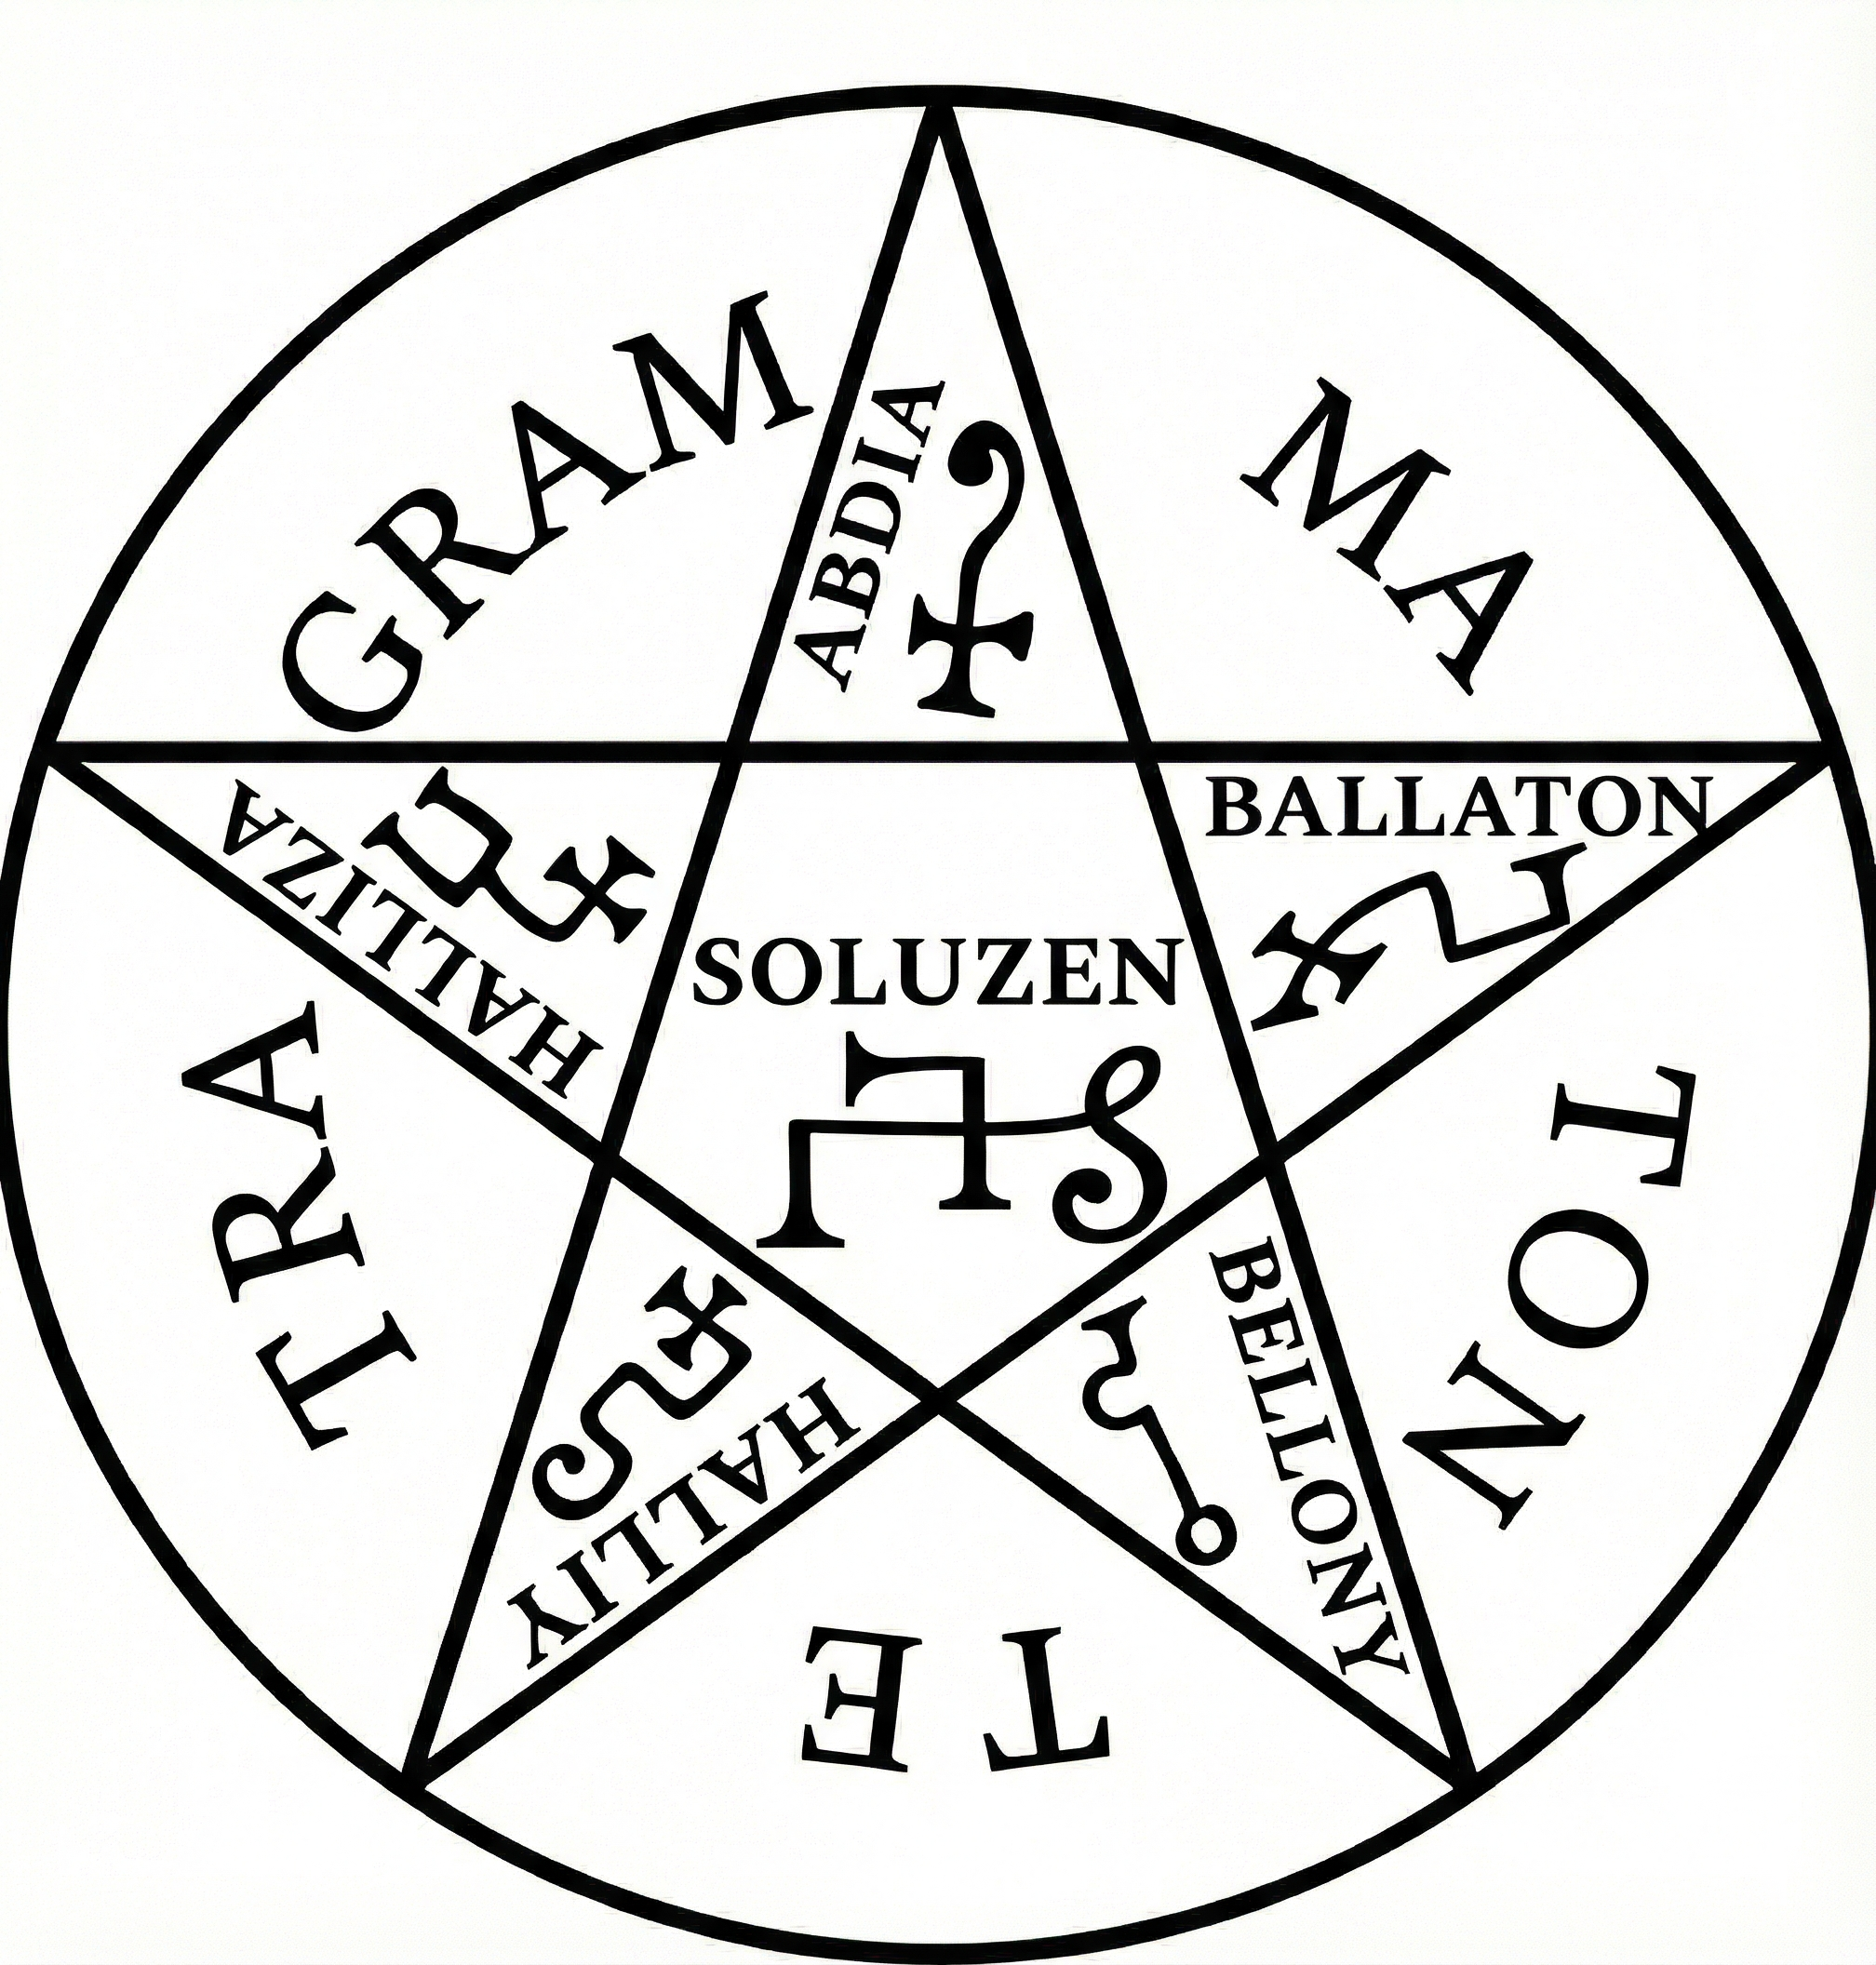
\includegraphics[width=\paperwidth,height=\paperheight,keepaspectratio]{solomon_pentagram.png}}
}

% --- METADATA ---
\title{Liber Defensionis}
\author{Michael Stilson}
\date{\today}

% --- THE DOCUMENT ---
\begin{document}
    % FRONT MATTER
    \pagenumbering{roman}
    
    % Frontispiece (Optional, if you want it back)
    % \thispagestyle{empty}
    % \vspace*{\fill}
    % \begin{center}
    %    \includegraphics[width=0.8\textwidth,keepaspectratio]{solomon_circle_and_triangle.png}
    % \end{center}
    % \vspace*{\fill}
    % \clearpage

	\maketitle
	\thispagestyle{empty}
	\vspace{1.0in}
	\begin{center}
		{\large
			A Practical Grimoire of Protection, Entrapment, and Expulsion \\
			\bigskip
			Derived from the Ars Goetia, Babylonian Tradition,
			and Roman Catholic Ritual
		}
	\end{center}
    \clearpage
    \tableofcontents
    \listoffigures
    \listoftables
    \clearpage

    % MAIN CONTENT (The Fragments)
    \pagenumbering{arabic}
    
    % Use \include for chapters (creates a page break automatically)
    \section{INTRODUCTION}
	\paragraph{}
		Herein is contained the \textit{Liber Defensionis}, a fortress of spirit constructed from three ancient foundations: the \textit{Ars Goetia} (The Lesser Key of Solomon), the Babylonian protective rites of the \textit{Udug-\d{h}ul}, and the exorcistic authority of the \textit{Rituale Romanum}.

		While these traditions span millennia and vast theological divides, they share a single, immutable principle: the invocation of Supreme Divine Authority to compel the obedience of lesser spiritual entities.

		The Goetic system (\cite{mathersgoetia1904}) is famously known for the conjuration of spirits, yet hidden within its circles and triangles lies a perfect defensive architecture. The magician was never intended to stand naked before the abyss; the system provides the names of compulsion, the seals of binding, and the geometry of containment. This work inverts the summoner's logic: rather than opening a door to call a spirit \textit{in}, we utilize the keys to lock the spirit \textit{out}.

		Complementing this geometry is the primal authority of the Babylonian tradition. Drawing from the \textit{En\={u}ma Eli\v{s}}, we utilize the Fifty Names of Marduk. In the ancient \textit{Marduk’s Address to the Demons}, the \textit{\={a}\v{s}ipu} (exorcist) did not merely pray to the god—he \textit{became} the god, speaking with the voice of the one who slew the chaos-dragon Ti\={a}mat.

		Finally, we anchor these ancient forms in the spoken authority of the Roman Catholic tradition, utilizing the \textit{Vade Retro Satana} and the \textit{Prayer to St. Michael}, formulas tempered by centuries of liturgical use against spiritual oppression.

		\paragraph{A Note on Illustrations}
		The geometric figures presented in this work follow the rectified schematics of \textcite{mathersgoetia1904} for the sake of operational clarity. The reader should note that the original 17\textsuperscript{th} century manuscripts, as critically examined by \textcite{peterson2001}, depict these seals in significantly more fluid, hand-drawn styles. We rely on the Victorian geometric precision here strictly for the construction of stable defensive barriers.\bigskip

		\noindent \textbf{The Structure of the Work:}

		\begin{description}
			\item[PART I: Repulsion] \hfill \\
			The establishment of barriers to prevent entry.
			\item[PART II: Entrapment] \hfill \\
			The geometry of containment for localized disturbances.
			\item[PART III: Expulsion] \hfill \\
			The rites of driving out that which has already embedded itself.
			\item[PART IV: The Fifty Names of Marduk] \hfill \\
			The assumption of Babylonian divine authority.
			\item[PART V: Roman Catholic Formulas] \hfill \\
			The traditional litanies of Christian exorcism.
		\end{description}
\clearpage


    	\section{REPULSION}
	\hspace{1cm}{\large Preventing Entry and Establishing Defensive Barriers}
	
	\subsection{The Core Logic}
	\paragraph{}
	The Ars Goetia operates on a hierarchy of names and symbols that assert divine authority over all 72 spirits.  The generalized elements are more powerful than individual spirit sigils because they invoke the source of authority rather than targeting an individual entity.  It is like having a master key instead of 72 separate keys.
	
	\subsection{Universal Names of Compulsion}
	These names from the Goetic conjurations work against all spirits of the hierarchy:
	
\begin{flushleft}
	\begin{xltabular}{\textwidth}{|l|X|}
		\hline
		\textbf{Name} & \textbf{Function} \\ \hline
		\endfirsthead
		\hline
		\textbf{Name} & \textbf{Function} \\ \hline
		\endhead
		
		TETRAGRAMMATON & Supreme divine authority (YHVH) \\ \hline
		ADONAI & Lordship and mastery \\ \hline
		AGLA & Protective barrier ("Thou art mighty forever, O Lord") \\ \hline
		PRIMEUMATON & First cause?commands origin \\ \hline
		ANAPHAXETON & Binds the hidden and formless \\ \hline
		EHYEH & "I Am" ? self?existent divine presence \\ \hline
		EL & God (generic, universal) \\ \hline
		ON & Being itself \\ \hline
		\caption{Universal Names of Compulsion}
		
	\end{xltabular}
\end{flushleft}

	\subsection{The Circle of Solomon}
	The original Circle of Solomon serves as the primary protective boundary.  Its key elements include:
	
	Outer Ring:
	
	\begin{itemize}
		\item The names EHYEH, KETHER, METATRON (divine name, sephirah, archangel)
		\item Four pentagrams at cardinal points
		\item Tau crosses (T) representing completion and sealing
	\end{itemize}
	Inner Ring:
	
	\begin{itemize}
		\item TETRAGRAMMATON (YHVH) repeated at quarters
		\item ADONAI inscribed between
	\end{itemize}
	Modification for pure defense: Close all gaps (the original has a \enquote{doorway} for the spirit
	to perceive the magician). Double the boundary lines.  Add AGLA between each pentagram.
	\begin{figure}[H]
		\centering
		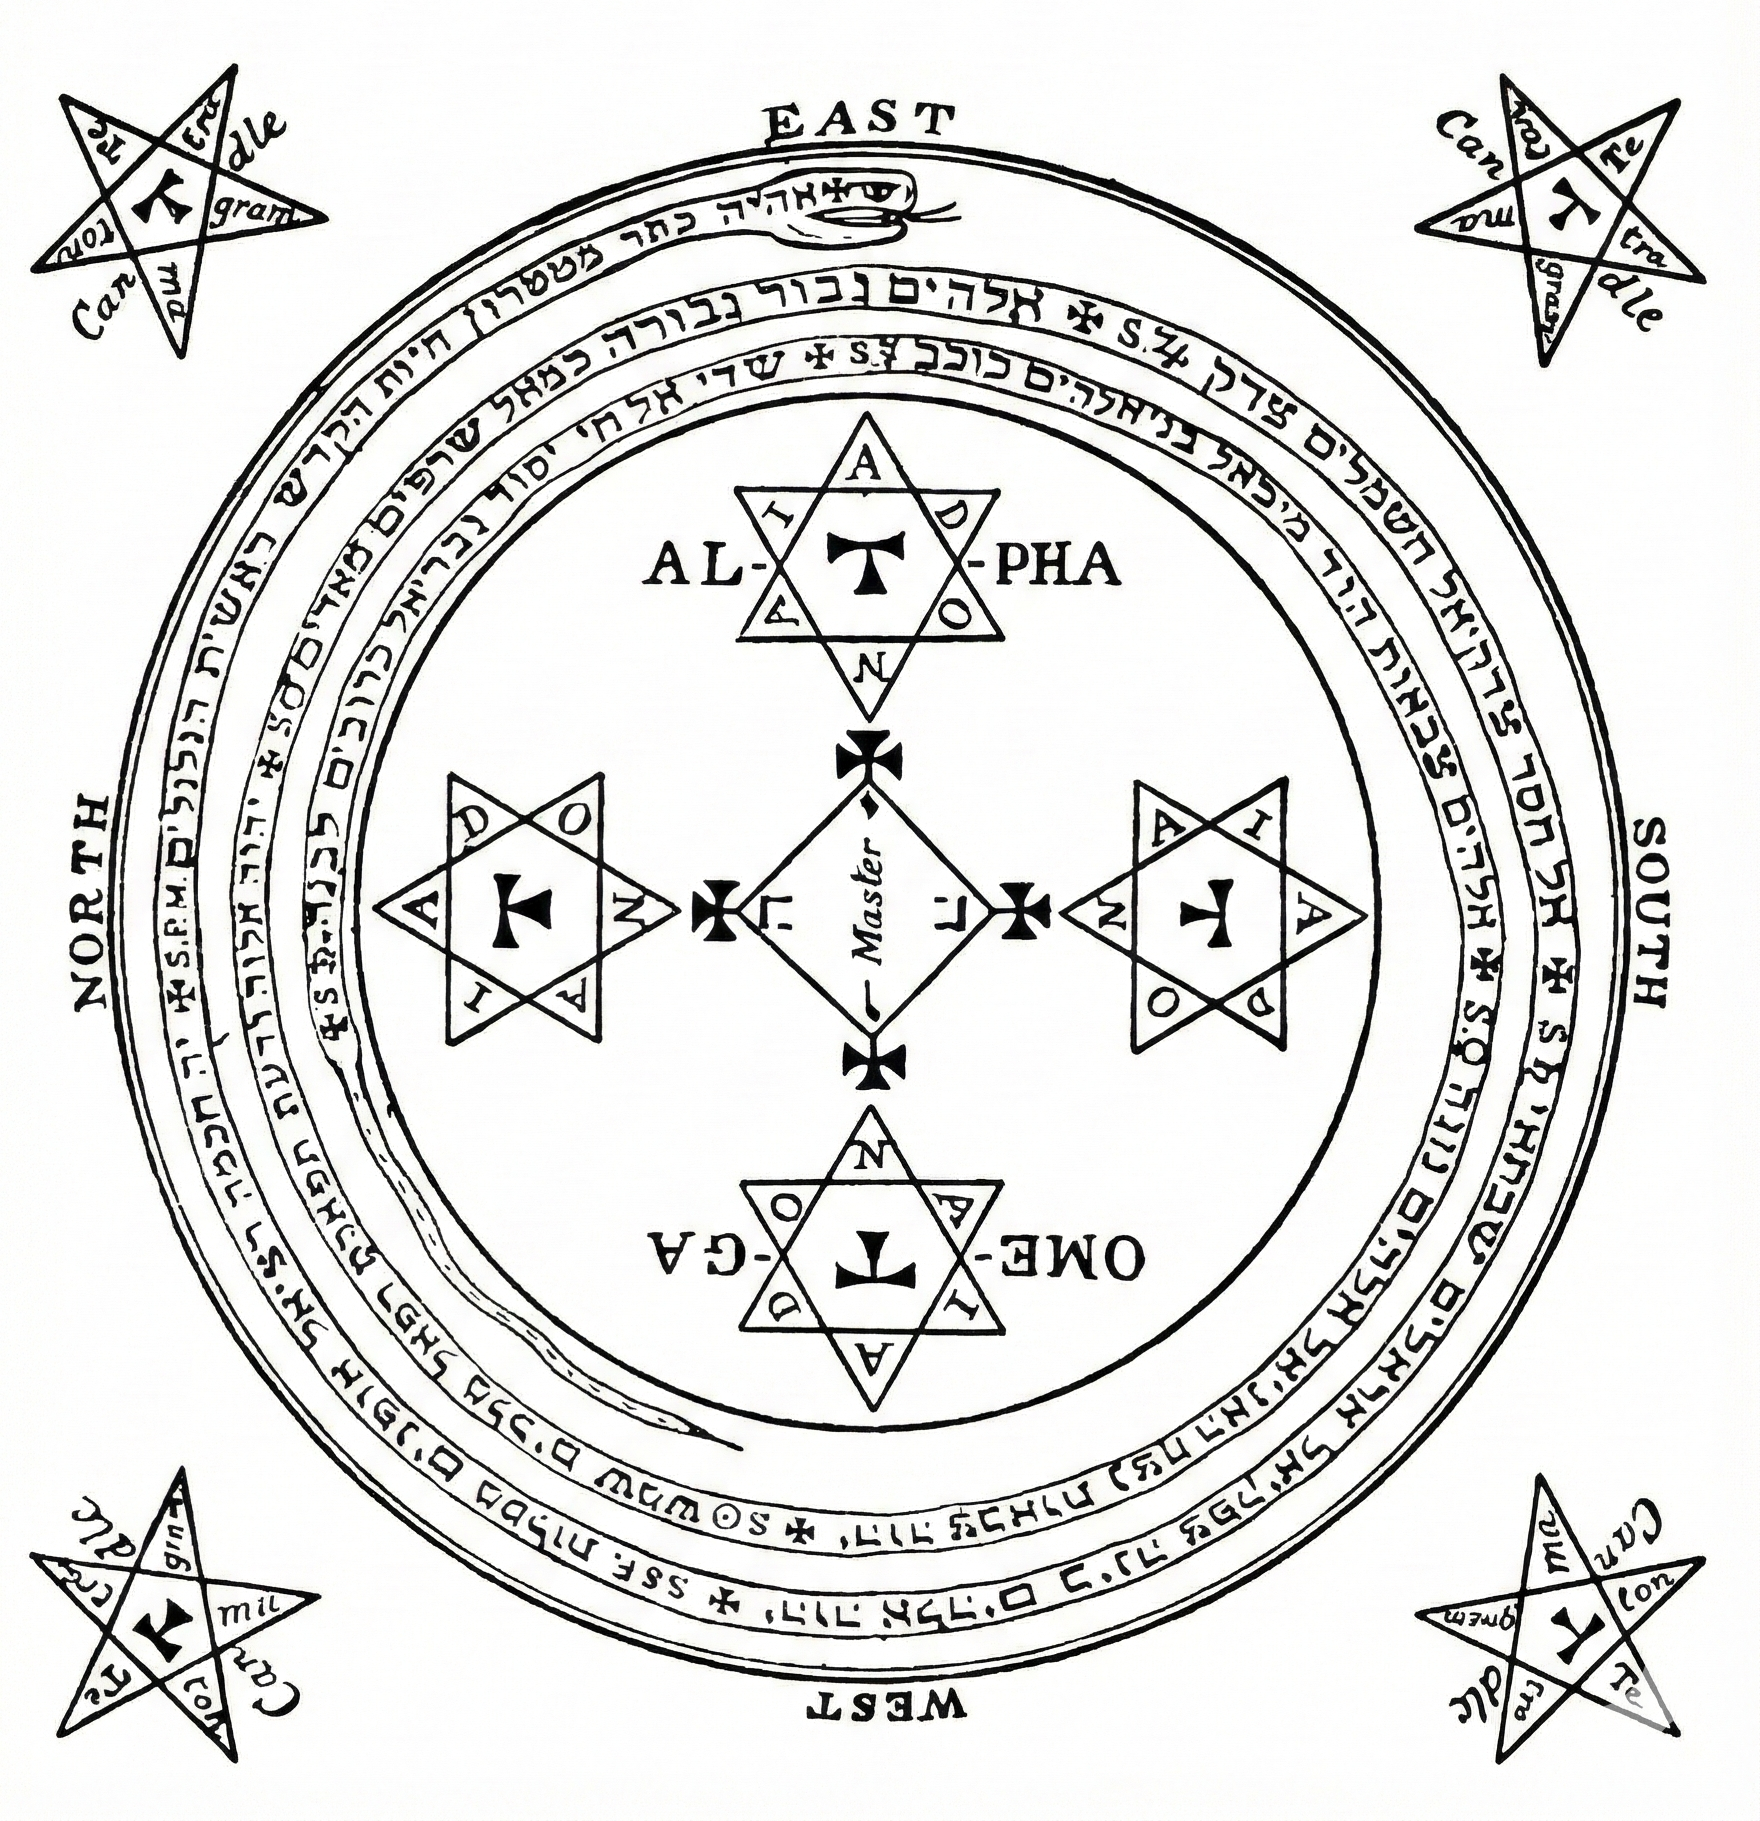
\includegraphics[width=0.3\paperwidth,keepaspectratio]{solomon_circle.png}
		\caption{The Circle of Solomon}
		\label{fig:solomoncircle}
	\end{figure}
	
	\subsection{The Triangle of Art (Repulsion Configuration)}
	For repulsion rather than summoning, the triangle's point faces OUTWARD from the protected space.  The three sides bear:
	\begin{figure}[H]
		\centering
		\includegraphics[width=0.3\paperwidth,keepaspectratio]{solomon_triangle.png}
		\caption{The Triangle of Art}
		\label{fig:solomontriangle}
	\end{figure}
	
	\begin{itemize}
		\item PRIMEUMATON (first moving)
		\item ANAPHAXETON (hidden one)
		\item TETRAGRAMMATON (the Name)
	\end{itemize}
	At the three points, inscribe MI-CHA-EL (Michael)---invoking the archangel who cast down rebellious spirits.  At center, place the Hexagram of Solomon containing no specific name, creating a \enquote{blank} binding that affects any entity.
	\begin{figure}[H]
		\centering
		\includegraphics[width=0.3\paperwidth,keepaspectratio]{solomon_hexagram.png}
		\caption{The Hexagram of Solomon}
		\label{fig:solomonhexagram}
		\cite[39]{mathersgoetia1904}
	\end{figure}
	
	\subsection{The Pentagram of Solomon}
	The most powerful generalized symbol in the system.  Originally worn by the magician for protection.
	\begin{figure}[H]
		\centering
		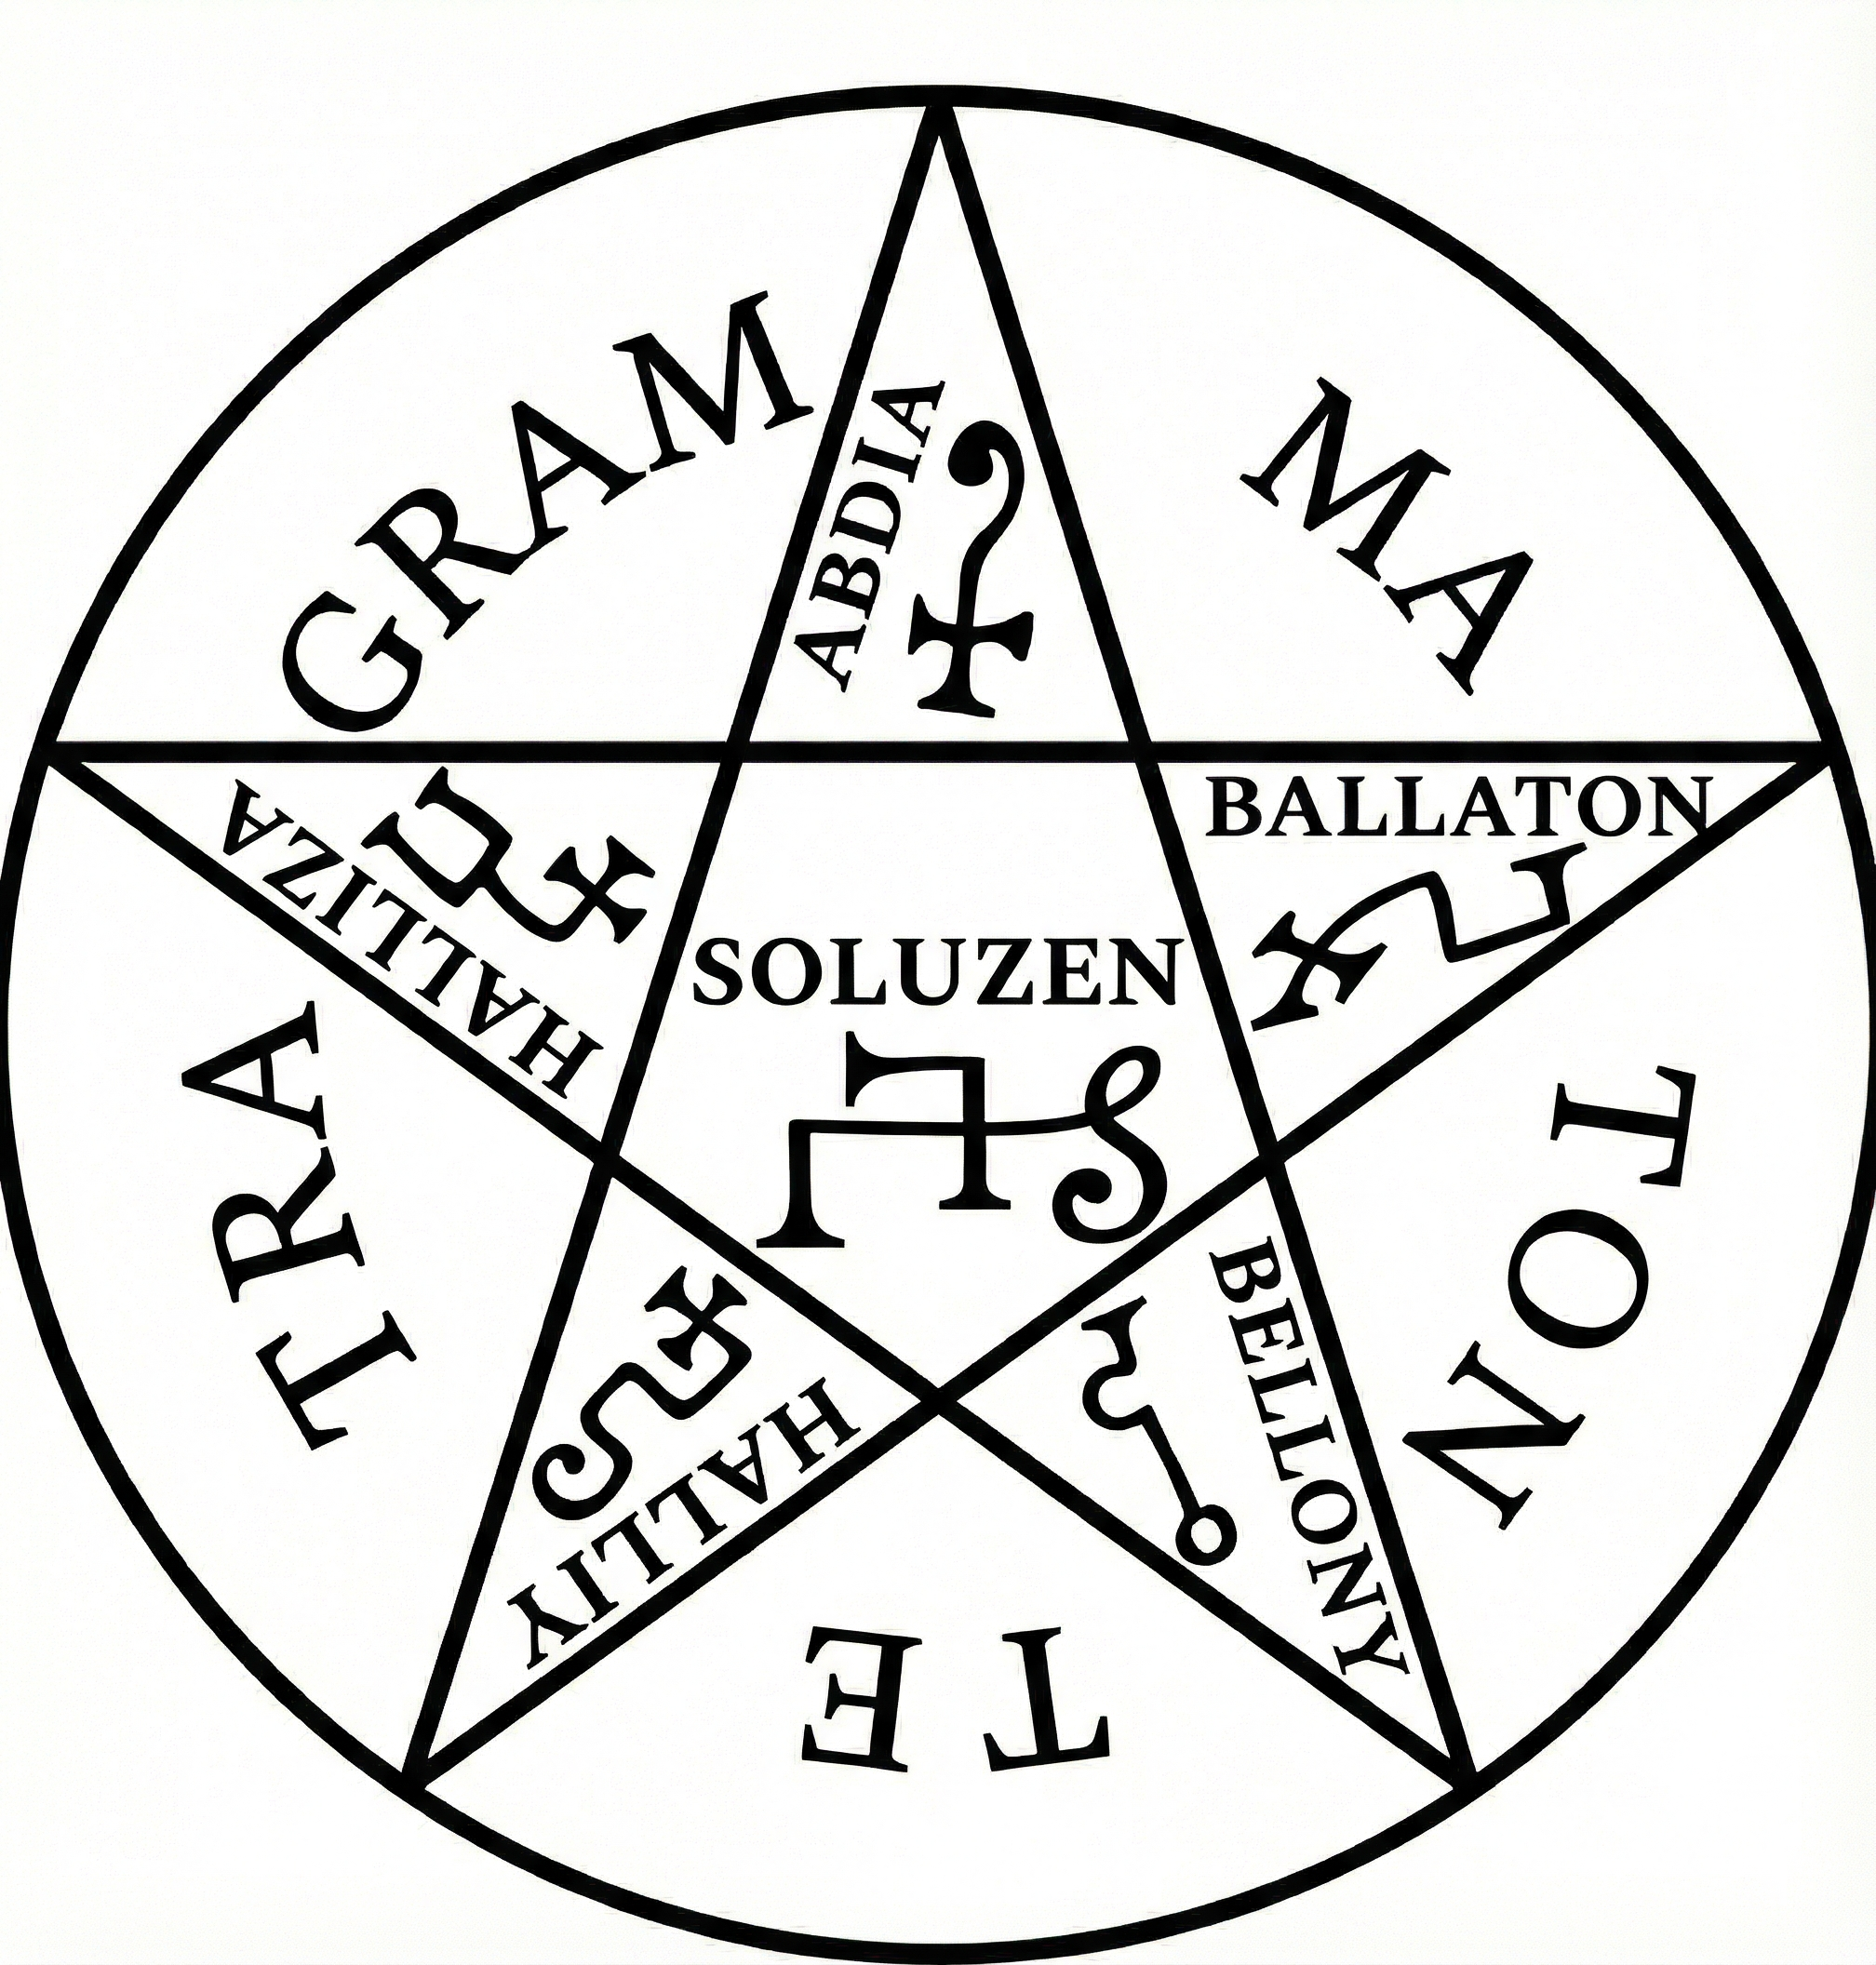
\includegraphics[width=0.3\paperwidth,keepaspectratio]{solomon_pentagram.png}
		\caption{The Pentagram of Solomon}
		\label{fig:solomonpentagram}
		\cite[39]{mathersgoetia1904}
	\end{figure}
	
	Elements:
	
	\begin{itemize}
		\item Five points: The five letters of YHShVH (Yahshuah---the \enquote{pentagrammaton})
		\item Center: The letters TE-TRA-GRAM-MA-TON arranged in the inner pentagon
		\item Outer ring: ABDIA, BALLATON, BELLONY, HALLIY, HALLIZA, SOLUZEN
	\end{itemize}
	For generalized repulsion: Inscribe on metal (traditionally copper or silver). Wear or mount at thresholds.  The symbol asserts authority over any of the 72 without needing to know which.
	
	\subsection{Combined Form}
	The union of the defensive circle and the constraining triangle creates the complete barrier.
	\begin{figure}[H]
		\centering
		\includegraphics[width=0.3\paperwidth,keepaspectratio]{solomon_circle_and_triangle.png}
		\caption[Circle and Triangle]{Circle and Triangle}
		\label{fig:circletriangle}
	\end{figure}

	\subsection{Spoken Formula for General Banishment}
	\begin{quotation}
	{\textquotedbl}By \gls{tetragrammaton}, ADONAI, AGLA, ON, EL---depart from this place.  By PRIMEUMATON who commands thy
	beginning and ANAPHAXETON who binds thy form---return to the depths appointed unto thee.{\textquotedbl}
	\end{quotation}
	
	
	\bigskip
	
	\clearpage


    \section{ENTRAPMENT}
\hspace{1cm}{\large Containing What Is Present and Localized}
\subsection{The Logic of Containment}
\paragraph{}{Repulsion prevents entry. Entrapment does the opposite—it creates a space the entity cannot leave. Where the Circle keeps things out, the trap keeps things in.}

The mechanism is attraction, not force. A correctly configured trap presents as a point of least resistance, a space where the entity's nature is accommodated rather than opposed. Once entered, the geometric boundary closes. The entity remains not because it is physically constrained, but because the exit requires a level of authority it does not possess.

This is critical: A trap does not work by overpowering the entity. It works by creating conditions the entity cannot navigate without external release.
\subsection{Entrapment vs. Repulsion: Key Differences}
\begin{xltabular}{\textwidth}{|X|X|}
	\hline
	\textbf{Repulsion} & \textbf{Entrapment} \\ \hline
	\endfirsthead
	\hline
	\textbf{Repulsion} & \textbf{Entrapment} \\ \hline
	\endhead
	Prevents approach & Draws in \\ \hline
	Closed boundary pointing outward & Open boundary that closes after entry \\ \hline
	Divine names assert dominance & Divine names establish inescapability \\ \hline
	Used preventatively & Used after intrusion detected \\ \hline
	Active resistance & Passive containment \\ \hline
	\caption{Repulsion vs. Entrapment}
\end{xltabular}
Understanding this distinction determines which tool to deploy. If the entity is outside and you want it to stay there: repulsion. If the entity is already present and you need to isolate it before expulsion: entrapment.
\subsection{The Triangle of Art: Trap Configuration}
\paragraph{}{The Triangle functions differently when used for entrapment rather than repulsion. The orientation reverses.}

\textbf{Configuration for Entrapment:}

Point the apex INWARD toward the suspected location of the entity. This creates a converging geometry that draws the entity toward the central point.
Inscribe the three sides with the same names as the repulsion configuration:
\begin{itemize}
	\item PRIMEUMATON (commands origin—the entity's beginning is bounded)
	\item ANAPHAXETON (binds the formless—prevents shapeshifting or dissolution)
	\item TETRAGRAMMATON (ultimate authority—no appeal, no escape)
\end{itemize}
Place the Hexagram of Solomon at the center, again without a specific sigil. The blank hexagram functions as a universal holding pattern.

\textbf{Deployment Procedure:}
\label{subsec:triangle-deployment}
\begin{enumerate}
	\item Identify the area of disturbance (window, mirror, doorway, object)
	\item Place the triangle over or around the affected area with apex pointing inward
	\item Drive iron nails into the ground at each of the three corners
	\item Place a small pile of salt at each point
	\item Light three black candles at the corners (black absorbs, does not repel)
	\item Speak the constraint formula (see below)
\end{enumerate}
\textbf{Constraint Formula:}
\begin{quotation}
	\enquote{By PRIMEUMATON at the first point, thy origin is sealed. By ANAPHAXETON at the second point, thy form is bound. By TETRAGRAMMATON at the third point, thy will is subject. Within this triangle thou art constrained. Thou canst not flee. Thou canst not hide. Thou must answer to the names of power inscribed herein.}
\end{quotation}
The constraint does not expel—it holds. Once the entity is trapped, expulsion protocols (Part III) can be applied with greater safety and efficacy.

\subsection{Physical Implements of Constraint}
\paragraph{}{The constraint formula above assumes the entity responds to verbal authority. When it does not—when the entity refuses to manifest, answer, or acknowledge the binding—physical implements provide direct compulsion.}

These are not symbolic tools. They function through sympathetic connection and material disruption of spiritual cohesion.

\textbf{The Hazel Wand (Scourge):}

Cut from hazel wood at dawn on a Tuesday or Saturday (Mars day for aggression, Saturn day for binding). The wand serves as both authority symbol and weapon.

\textit{Application:} If the constrained entity refuses to manifest or respond, strike the air within the triangle sharply with the wand. Three strikes, one at each corner. Each strike transmits force through the geometric boundary directly to the entity's form.

More aggressive: Strike the entity's sigil (if known) or any object associated with the disturbance. The blow creates sympathetic pain—not physical injury, but spiritual discomfort that compels compliance. This is documented in the \textit{Grimorium Verum} tradition as standard procedure when divine names alone prove insufficient \cite{peterson2001}.

\textbf{The Ring as Brand:}

The \textit{Testament of Solomon} (1st-3rd c.) describes the original function of the seal-ring: not protection, but \textit{dominance}. When the demon Ornias refused to obey, Solomon threw the ring bearing the Pentalpha directly at the spirit's manifestation. Contact with the seal branded the entity, asserting ownership.

\textit{Modern Application:} If working with a physical manifestation or strong localized presence, a seal-ring or metal disc bearing the Pentagram of Solomon can be thrown into the triangle's center or placed forcibly upon any object housing the entity. This is offensive constraint—establishing control through direct contact rather than geometric boundary.

\textbf{Iron Implements:}

Iron disrupts spiritual cohesion. The metal's properties create active discomfort rather than passive barrier.

\begin{itemize}
	\item \textit{Iron nails at triangle corners:} As specified in the deployment procedure (\S\ref{subsec:triangle-deployment}), iron nails driven at each corner anchor the geometric form and create material "stakes" that prevent the entity from dissolving or shifting form.
	\item \textit{Iron chain or wire:} Wrap around objects suspected of harboring the entity. Seven wraps minimum (seven being the number of binding in traditional practice).
	\item \textit{Iron blade:} Hold over the triangle or vessel while speaking the constraint. The presence of drawn iron intensifies the discomfort of containment.
\end{itemize}

\textbf{When to Escalate to Physical Methods:}

\begin{enumerate}
	\item Speak the Constraint Formula once.
	\item Wait. Give the entity opportunity to respond.
	\item If no response after reasonable time (several minutes): Strike the triangle corners with hazel wand.
	\item If still no response: Strike any physical focus (mirror, object, doorway) associated with the disturbance.
	\item If entity manifests but refuses to answer: Present drawn iron blade or place ring/seal directly into the manifestation's perceived location.
\end{enumerate}

This is escalation, not starting procedure. The verbal formula should always be attempted first. Physical compulsion is for when authority alone proves insufficient—and the texts acknowledge this happens.

\subsection{The Secret Seal of Solomon}
This seal appears in the Lemegeton as the mechanism by which spirits were bound into brass vessels \cite{peterson2001}. Its power is already generalized—it compels submission regardless of the entity's individual nature or rank.
The seal consists of:
\begin{itemize}
	\item Concentric circles forming a boundary
	\item A central square containing divine names (typically TETRAGRAMMATON and ADONAI)
	\item Hebrew letters arranged around the perimeter
	\item Geometric patterns that create a "lock" requiring specific knowledge to open
\end{itemize}
\textbf{Practical Applications:}
\begin{itemize}
	\item \textit{Threshold Installation:} Place beneath doorways or windows to trap entities attempting entry. The seal does not prevent passage—it captures what crosses.
	\item \textit{Container Lid:} Inscribe or affix to the lid of any vessel used for containment. Once sealed, the entity cannot escape without the seal being broken by external authority.
	\item \textit{Surface Inscription:} Carve into floors, walls, or objects where persistent disturbance is suspected. The seal binds what is present to that location.
\end{itemize}
\textbf{Activation:}
Unlike the Circle, which activates through spoken formula, the Secret Seal functions through physical closure. Once an entity is within its boundary, physically sealing the container or covering the inscription activates the binding. The seal must then be maintained—any break in the physical integrity compromises the trap.
\subsection{The Brass Vessel: Physical Containment}
\paragraph{}{The Lemegeton describes brass vessels for containing evoked spirits. For defensive work, the vessel serves as a portable trap—useful when an entity is bound to a specific object or when mobile containment is required.
}\textbf{Construction:}
\begin{itemize}
	\item \textit{Body:} Brass (copper-zinc alloy). Brass conducts spiritual force while remaining stable. Minimum size: large enough to contain the bound object if applicable, or at least 6 inches in diameter for formless entities.
	\item \textit{Lid:} Lead. Lead restricts and binds (associated with Saturn—limitation, endings). The Secret Seal of Solomon must be impressed, engraved, or affixed to the underside of the lid.
	\item \textit{Base:} Iron plate beneath the vessel. Iron disrupts spiritual cohesion and prevents the entity from "sinking" through the bottom.
	\item \textit{Interior contents (optional but recommended):}
	\begin{itemize}
		\item Mercury in sealed glass vial (fluidity bound—prevents shapeshifting)
		\item Graveyard earth (association with the dead—grounds formless entities)
		\item Salt (purification and binding)
		\item Sulfur (traditional binding agent in alchemical work)
	\end{itemize}
\end{itemize}
\textbf{Usage Procedure:}
\begin{enumerate}
	\item If the entity is bound to an object: place the object inside the vessel
	\item If the entity is formless: use the Triangle of Art to constrain it to a specific location, then position the open vessel at the center of the triangle
	\item Speak the binding: \enquote{By the authority of Solomon who bound thy kind, by the Secret Seal impressed upon this vessel, by the names of power that compel thee—ENTER this vessel and be bound therein.}
	\item Seal the vessel immediately with the lead lid (Secret Seal facing inward)
	\item Bind the vessel with iron wire or chain, wrapping at least seven times
	\item Store in a location away from human habitation, preferably buried or encased in concrete
\end{enumerate}
\textbf{Warning:}
Once sealed, the vessel should not be opened except under controlled conditions with full protective protocols in place. The binding does not destroy the entity—it contains it. Breaking the seal releases what is inside.
\subsection{When to Use Each Method}
\begin{xltabular}{\textwidth}{|l|X|X|}
	\hline
	\textbf{Method} & \textbf{Use Case} & \textbf{Limitation} \\ \hline
	\endfirsthead
	\hline
	\textbf{Method} & \textbf{Use Case} & \textbf{Limitation} \\ \hline
	\endhead
	Triangle & Localized disturbance; entity present but not yet expelled & Temporary. Must be followed by expulsion or vessel containment. \\ \hline
	Secret Seal & Threshold protection; binding entity to specific location & Stationary. Only works where physically installed. \\ \hline
	Brass Vessel & Portable containment; object-bound entities; when expulsion is not possible & Permanent containment required. Must be maintained. \\ \hline
	\caption{Entrapment Methods}
\end{xltabular}
The Triangle isolates. The Seal binds. The Vessel contains. In practice, these methods often work in sequence: Triangle constrains, Seal reinforces, Vessel provides final containment if expulsion fails.
\subsection{Combining Entrapment with Expulsion}
Entrapment is not an end state—it is a control measure. Once the entity is contained within the Triangle or Vessel, expulsion protocols (Part III) can be applied with reduced risk. The entity cannot flee, cannot hide, and is forced to respond to the escalating conjurations.
This is the proper sequence for embedded or persistent intrusions:
\begin{enumerate}
	\item Constrain with Triangle
	\item Apply First Conjuration (command)
	\item If unsuccessful, reinforce with Secret Seal
	\item Apply Second Conjuration (threat)
	\item If still unsuccessful, transfer to Vessel
	\item Apply Third Conjuration (curse) with Babylonian or Catholic formulas as escalation
\end{enumerate}
Containment creates the conditions for effective expulsion. Without it, the entity may simply withdraw temporarily and return later.

    	\section{EXPULSION}
\begin{center}
		{\large Driving Out What Is Already Embedded}
\end{center}	

	\subsection{Identifying the Attachment Type}
	Before expulsion, determine what the entity is attached to:
	
	\begin{flushleft}
		
		\begin{xltabular}{\textwidth}{|Y|Y|Y|}
			\hline
			\textbf{Locational} & \textbf{Object-Bound} & \textbf{Personal} \\ \hline
			\endhead
			Activity in specific areas; doesn't follow people who leave &
			Disturbance centers on item; stops when item removed &
			Follows person; effects persist outside location \\ \hline
			\emph{Solution}: Space cleansing and reconsecration &
			\emph{Solution}: Destroy or seal the object &
			\emph{Solution}: Personal severance ritual \\ \hline
			\caption{Attachment Type}
		\end{xltabular}
	\end{flushleft}
	\subsection{The Three Conjurations}
	\paragraph{}{The Goetic system escalates through increasingly severe conjurations.  Each level invokes higher powers and threatens greater consequences.
	}
	\subsubsection{First Conjuration (Command)}
	\begin{quotation}
	\enquote{I conjure and command thee, spirit present in this place, by the living God, by the true God, by the holy God, by the God who spoke and all was made, who commanded and all was created.  I conjure thee by TETRAGRAMMATON YHVH, who cast Adam from Eden, who brought the Flood upon the world, who consumed Sodom with fire, who parted the Red Sea.  I conjure thee by ADONAI, Lord of all creation, by EHYEH ASHER EHYEH, I Am That I Am, by EL SHADDAI, God Almighty, by ELOHIM GIBOR, God of Strength.  Thou art bound by these names.  Thou shalt not remain where thou art not welcome.  Thou shalt depart unto the place appointed thee.  By what name art thou called? By what authority didst thou enter? I command thee: SPEAK.}
	\end{quotation}
	
	\subsubsection{Second Conjuration (Threat)}
	\begin{quote}If resistance or silence, escalate:\end{quote}
	
	\begin{quotation}
	\enquote{Spirit, thou hast not obeyed.  I conjure thee now by the dreadful Day of Judgment, by the Sea of Glass before the throne, by the Four Beasts with eyes before and behind, by the fire about the throne, by the holy angels of heaven, by the mighty wisdom of God.  I conjure thee by TETRAGRAMMATON YHVH, by ADONAI, EHYEH, EL, ELOHIM, by SADAY, ZEBAOTH, ELION, by ESCERCHIE, ORISTON, JAH, TETRAGRAMMATON.  If thou dost not obey, I will curse thee unto the depths of the abyss.  I will bind thee in chains of darkness.  I will trip from thee all rank and power.  DEPART.  NOW.  Unto the place from whence thou came.  Return not to this place, nor to any whom I protect.  By AGLA, be GONE.}
\end{quotation}
	
	\subsubsection{Third Conjuration (Curse)}
	\begin{quote}Final escalation with the four archangels:\end{quote}
	
	\begin{quotation}
	\enquote{Disobedient and obstinate spirit, because thou hast not heeded the words of power, because thou hast defied the names of God, I curse thee in the name of TETRAGRAMMATON.  By ANAPHAXETON, I strip thy hidden protections.  By PRIMEUMATON, I sever thy connection to this place.  By TETRAGRAMMATON, I cast thee out utterly.  MICHAEL stands at the East with sword drawn.  GABRIEL stands at the West with the cup of banishment.  RAPHAEL stands at the South with the winds of driving.  URIEL stands at the North with flames of purification.  There is no quarter for thee.  There is no refuge.  I expel thee by the power of the Most High.  I expel thee by Solomon who bound thy kind.  I expel thee by the Seal that commands thy obedience.  GO.  TETRAGRAMMATON compels thee.  ADONAI compels thee.  AGLA compels thee.  EL.  YAH.  YHVH.  EHYEH.  SADAY.  BE GONE FROM THIS PLACE FOREVER.}
\end{quotation}
	
	\subsection{Severance Procedures}
	For Locational Attachment:
	
	\begin{enumerate}
		\item Take iron blade or nail
		\item Beginning at center of disturbance, \enquote{cut} the air in a cross pattern
		\item Speak: \enquote{I sever thy tie to this place.}
		\item Move to each corner of the room/space, repeat
		\item At threshold, cut horizontally across doorway: \enquote{Thy passage here is ended.}
	\end{enumerate}
	For Object Attachment:
	
	Option A --- Destruction: Remove object to crossroads or running water.  Break it while speaking: \enquote{By TETRAGRAMMATON, I break thy vessel.  By ADONAI, I release thy hold.  By AGLA, I end thy presence.} Bury fragments in separate locations or burn and scatter ashes in running water.
	
	Option B --- Sealing: Place in brass vessel with lead lid.  Seal with Secret Seal of Solomon.  Bind with iron chain or wire.  Bury deeply or encase in concrete.
	
	For Personal Attachment:
	
	\begin{enumerate}
		\item Person stands in center of Circle of Solomon
		\item Operator works from outside, with hazel wand
		\item Beginning at crown of head, move wand downward: \enquote{From thy head, depart.}
		\item At throat: \enquote{From thy voice, depart.}
		\item At heart: \enquote{From thy heart, depart.}
		\item At hands: \enquote{From thy works, depart.}
		\item At feet: \enquote{From thy path, depart.}
		\item Final sweep, head to toe, with full severance declaration
		\item Person is anointed with protective oil and given Pentagram of Solomon to wear
	\end{enumerate}
	
	\bigskip
	
	\clearpage


    	\section{THE FIFTY NAMES OF MARDUK}
	\hspace{1cm}{\large Babylonian Divine Authority for Exorcism}
	
	\subsection{Origin and Function}
	The Fifty Names of Marduk derive from the Babylonian creation epic, the {Enuma Elish}{\index{Enuma Elish}} (circa 12\textsuperscript{th} century BCE). These names appear in Tablets VI and VII and represent powers given to Marduk after his victory over the chaos dragon Ti\={a}mat.
	
	These names were used in \enquote{Marduk's Address to the Demons,{\textquotedblright} a key section of the ancient Mesopotamian exorcism series \index{Udug-\d{h}ul}Udug-\d{h}ul ({\textquotedblleft}Evil Demons}). When performing exorcisms, the exorcist (\=a\v{s}ipu) would essentially become Marduk, speaking in the first person as Asallu\d{h}i/Marduk.
	
	The core principle: By reciting the Fifty Names, the exorcist assumes the identity and authority of Marduk himself---the god who defeated primordial chaos.
	
\subsection{The Fifty Names}
\begin{xltabular}{\textwidth}{|c|l|X|}
	\hline
	\textbf{\#} & \textbf{Name} & \textbf{Domain/Power} \\ \hline
	\endfirsthead
	\hline
	\textbf{\#} & \textbf{Name} & \textbf{Domain/Power} \\ \hline
	\endhead
	
	1 & \textsc{Marduk} & The Son of the Sun; he who establishes cosmic order. \\ \hline
	2 & \textsc{Marukka} & He who creates the wisdom of all. \\ \hline
	3 & \textsc{Marutukku} & Master of the arts of protection; hostile to the aggressor. \\ \hline
	4 & \textsc{Barashaku\v{s}u} & He who compelled the obedient into chaos; he who is wide of heart. \\ \hline
	5 & \textsc{Lugaldimmerankia} & Master of Order, who puts the wind demons to flight. \\ \hline
	6 & \textsc{Nari} & The Director, who regulates the heavens and earth. \\ \hline
	7 & \textsc{Asallu\d{h}i} & The Name of Power; the protector of the good, the banisher of the wicked. \\ \hline
	8 & \textsc{Namtila} & The Life-Giver; he who restores the dead to life. \\ \hline
	9 & \textsc{Namru} & The Bright One; he who purifies the path. \\ \hline
	10 & \textsc{Asaru} & Bestower of cultivation; who establishes the water levels. \\ \hline
	11 & \textsc{Asarualim} & He whose counsel is esteemed; the light of the gods. \\ \hline
	12 & \textsc{Asarualimnunna} & The Power that presides over the armor of the gods. \\ \hline
	13 & \textsc{Tutu} & He who silences the weeping; the supreme banisher. \\ \hline
	14 & \textsc{Ziukkina} & Life of the Host; he who establishes the heavens. \\ \hline
	15 & \textsc{Ziku} & The God of the Breath; Lord of Holiness. \\ \hline
	16 & \textsc{Agaku} & The Lord of the Charm; he who brings the dead to life. \\ \hline
	17 & \textsc{Tuku} & The Lord of the Ban; he whose spell is holy. \\ \hline
	18 & \textsc{\v{S}azu} & He who knows the heart; the searcher of souls. \\ \hline
	19 & \textsc{Zisi} & The Reconciler; the silencer of the enemy. \\ \hline
	20 & \textsc{Su\d{h}rim} & He who roots out the enemies with the weapon. \\ \hline
	21 & \textsc{Su\d{h}gurim} & He who destroys the foes; who makes the shell to vanish. \\ \hline
	22 & \textsc{Za\d{h}rim} & The Destroyer; he who grinds the enemy to dust. \\ \hline
	23 & \textsc{Za\d{h}gurim} & He who destroys the enemy in a specific way (the specialized destroyer). \\ \hline
	24 & \textsc{Enbilulu} & The Lord of the Abundance; he who governs the waters. \\ \hline
	25 & \textsc{Epadun} & The Lord of the Plain; who irrigates the fields. \\ \hline
	26 & \textsc{Gugal} & The Inspector of the Canals; the Lord of the Overflow. \\ \hline
	27 & \textsc{Hegal} & He who accumulates the harvest; who brings rain. \\ \hline
	28 & \textsc{Sirsir} & He who heaps up the mountain (of grain) upon the serpent. \\ \hline
	29 & \textsc{Mala\d{h}} & The Boatman; he who navigates the ship of state. \\ \hline
	30 & \textsc{Gil} & The Storehouse; the seed-preserver. \\ \hline
	31 & \textsc{Gilma} & The Founder; who renders the firmament permanent. \\ \hline
	32 & \textsc{Agilma} & The Lofty One; who removes the hoop (of constraint). \\ \hline
	33 & \textsc{Zulum} & The Divider; who assigns the fields. \\ \hline
	34 & \textsc{Mummu} & The Creator of the Universe; the One who was before. \\ \hline
	35 & \textsc{Zulummar} & The Hammer; he who crushes the opposition. \\ \hline
	36 & \textsc{Lugalabdubur} & The Destroyer of the Gods of Ti\={a}mat; the conqueror. \\ \hline
	37 & \textsc{Pagalguenna} & The Leader of all Lords; whose spirit is pre-eminent. \\ \hline
	38 & \textsc{Lugaldurma\d{h}} & The King of the Bond of the Gods; the Lord of the Link. \\ \hline
	39 & \textsc{Aranunna} & The Counselor of Ea; the creator of the treaty. \\ \hline
	40 & \textsc{Dumuduku} & The Son of the Holy Mound; the place of renewal. \\ \hline
	41 & \textsc{Lugalanna} & The King of the Height; the Lord of the Strength. \\ \hline
	42 & \textsc{Lugalugga} & The Lord of the Hosts of the Dead; he who extracts the life. \\ \hline
	43 & \textsc{Irkingu} & He who carried off the Kingu (Dragon-General) in the battle. \\ \hline
	44 & \textsc{Kinma} & The Judge and Governor of the Gods; the director of names. \\ \hline
	45 & \textsc{Esizkur} & He who sits in the House of Prayer; the hearer of vows. \\ \hline
	46 & \textsc{Gibi} & The One who maintains the Point; the creator of the winds. \\ \hline
	47 & \textsc{Addu} & The Storm King; who covers the sky with his shroud. \\ \hline
	48 & \textsc{A\v{s}aru} & The Overseer; who regulates the gods of destiny. \\ \hline
	49 & \textsc{Nebiru} & The Star of the Pole; he who holds the pivot of the stars. \\ \hline
	50 & \textsc{Nibbura} & Father Enlil bestowed this name: The Lord of the Lands. \\ \hline
	\caption[The Fifty Names of Marduk]{The Fifty Names of Marduk \\ \cite{speiser1969}}
	\end{xltabular}
	
	\subsection{Using the Names in Exorcism}
	The exorcist declares each name in the first person, assuming Marduk's identity:
	
	\enquote{I am Asallu\d{h}i, magician of the gods.  I am MARDUK, supreme authority.  I am ASARULUDU, wielder of the flaming sword.  I am NAM\-TIL\-LA\-KU, who speaks with spirits.  I am LUG\-GAL\-DIM\-MER\-ANK\-IA, who commands the wind demons and puts order into chaos.  By these names, I command thee: DEPART.}
	
	
	\bigskip
	
	\clearpage


    \section{ROMAN CATHOLIC FORMULAS}
\begin{center}
	{\large Traditional Christian Exorcism Prayers}
\end{center}

\subsection{The Protective Briefs}
\rubric{Note on Usage}
These formulas are distinct from the prayers of exorcism below in that they are often worn as physical talismans (apamaic texts) or inscribed on medals, rather than spoken as a long-form liturgy.

% ==========================================
% 1. THE MEDAL OF ST. BENEDICT
% ==========================================
\subsubsection*{i. The Vade Retro Satana}
This medieval Western Christian formula (1415) is traditionally associated with the Medal of Saint Benedict.

% --- IMAGE PLACEHOLDER ---
\begin{figure}[H]
	\centering
	\includegraphics[width=0.3\paperwidth,keepaspectratio]{benedict_face.png}
	\label{fig:benedict_medal_face}
\end{figure}
\begin{figure}[H]
	\centering
	\includegraphics[width=0.3\paperwidth, keepaspectratio]{benedict_cross.png}
	\caption{The Medal of Saint Benedict \cite{stutler_medal}}
	\label{fig:benedict_medal_cross}
\end{figure}
% --- PART 1: THE INSCRIPTIONS ---
\rubric{The Inscriptions (The Cross)}

\begingroup
\centering
% PAX
{\latinfont\Huge\textbf{PAX} \par}
{\itshape\footnotesize PEACE \par}

\vspace{1em}

% CSPB - Uses \medalcross (The Object)
{\latinfont\Large\textbf{C. \medalcross\ S. P. B.} \par}
{\footnotesize (Crux Sancti Patris Benedícti) \par}

\vspace{0.5em}

{\itshape\footnotesize The Cross of Our Holy Father Benedict \par}
\endgroup

\vspace{1.5em}

% --- PART 2: THE FORMULA ---
\rubric{The Formula (The Rim)}
\textit{\small To be recited while making the Sign of the Cross at the markers (\rubriccross).}

\begingroup
\centering
% LATIN - Uses \rubriccross (The Action)
{\latinfont\Large
	Crux sácra sit míhi lux \rubriccross \par
	Non dráco sit míhi dux \rubriccross \par
	Váde rétro Sátana! \par
	Númquam suáde míhi vána \rubriccross \par
	Sunt mála quae líbas \par
	Ípse venéna bíbas \rubriccross \par}

\vspace{1em}

% ENGLISH
{\itshape\small
	May the Holy Cross be my light!
	May the dragon never be my guide!
	Begone, Satan!
	Never tempt me with your vanities!
	What you offer is evil.
	Drink the poison yourself! \par}
\endgroup

\vspace{2em}
\hrule width 0.5\textwidth \relax
\vspace{2em}

% ==========================================
% 2. THE BRIEF OF ST. ANTHONY
% ==========================================
\subsubsection*{ii. The Brief of Saint Anthony}
Known as the \textit{Ecce Crucem Domini}, this brief is often inscribed on parchment or linen shaped like a small shield.

\begin{figure}[H]
	\centering
	\includegraphics[width=0.3\paperwidth, keepaspectratio]{st_anthony_brief_shield.png}
	\caption{The Brief of Saint Anthony}
	\label{fig:st_anthony_brief}
\end{figure}
\begin{figure}[H]
	\centering
	\includegraphics[width=0.3\paperwidth, keepaspectratio]{st_anthony_brief_cross.jpg}
	\caption{Traditional St. Anthony Brief Cross \cite{anthony_brief_source}}
	\label{fig:anthony_cross}
\end{figure}

\rubric{The Invocation}

\begingroup
\centering
% LATIN - Versicle and Response
{\latinfont\Large
	\V Ecce Crucem Dómini! \rubriccross \par
	\R Fúgite pártes advérsae! \par
	\vspace{0.5em}
	\V Vícit Leo de tríbu Júda, \par
	\R Radix Dávid! Allelúia! \par
}

\vspace{1em}

% ENGLISH
{\itshape\small
	\V Behold the Cross of the Lord! \par
	\R Flee, ye hostile powers! \par
	\V The Lion of the tribe of Judah, \par
	\R The Root of David, has conquered! Alleluia! \par}
\endgroup

\newpage

% ==========================================
% 3. PRAYER TO SAINT MICHAEL
% ==========================================
\subsection{Prayer to Saint Michael the Archangel}
Introduced by Pope Leo XIII in 1886. The short version is used for general protection.


\begin{figure}[H]
	\centering
	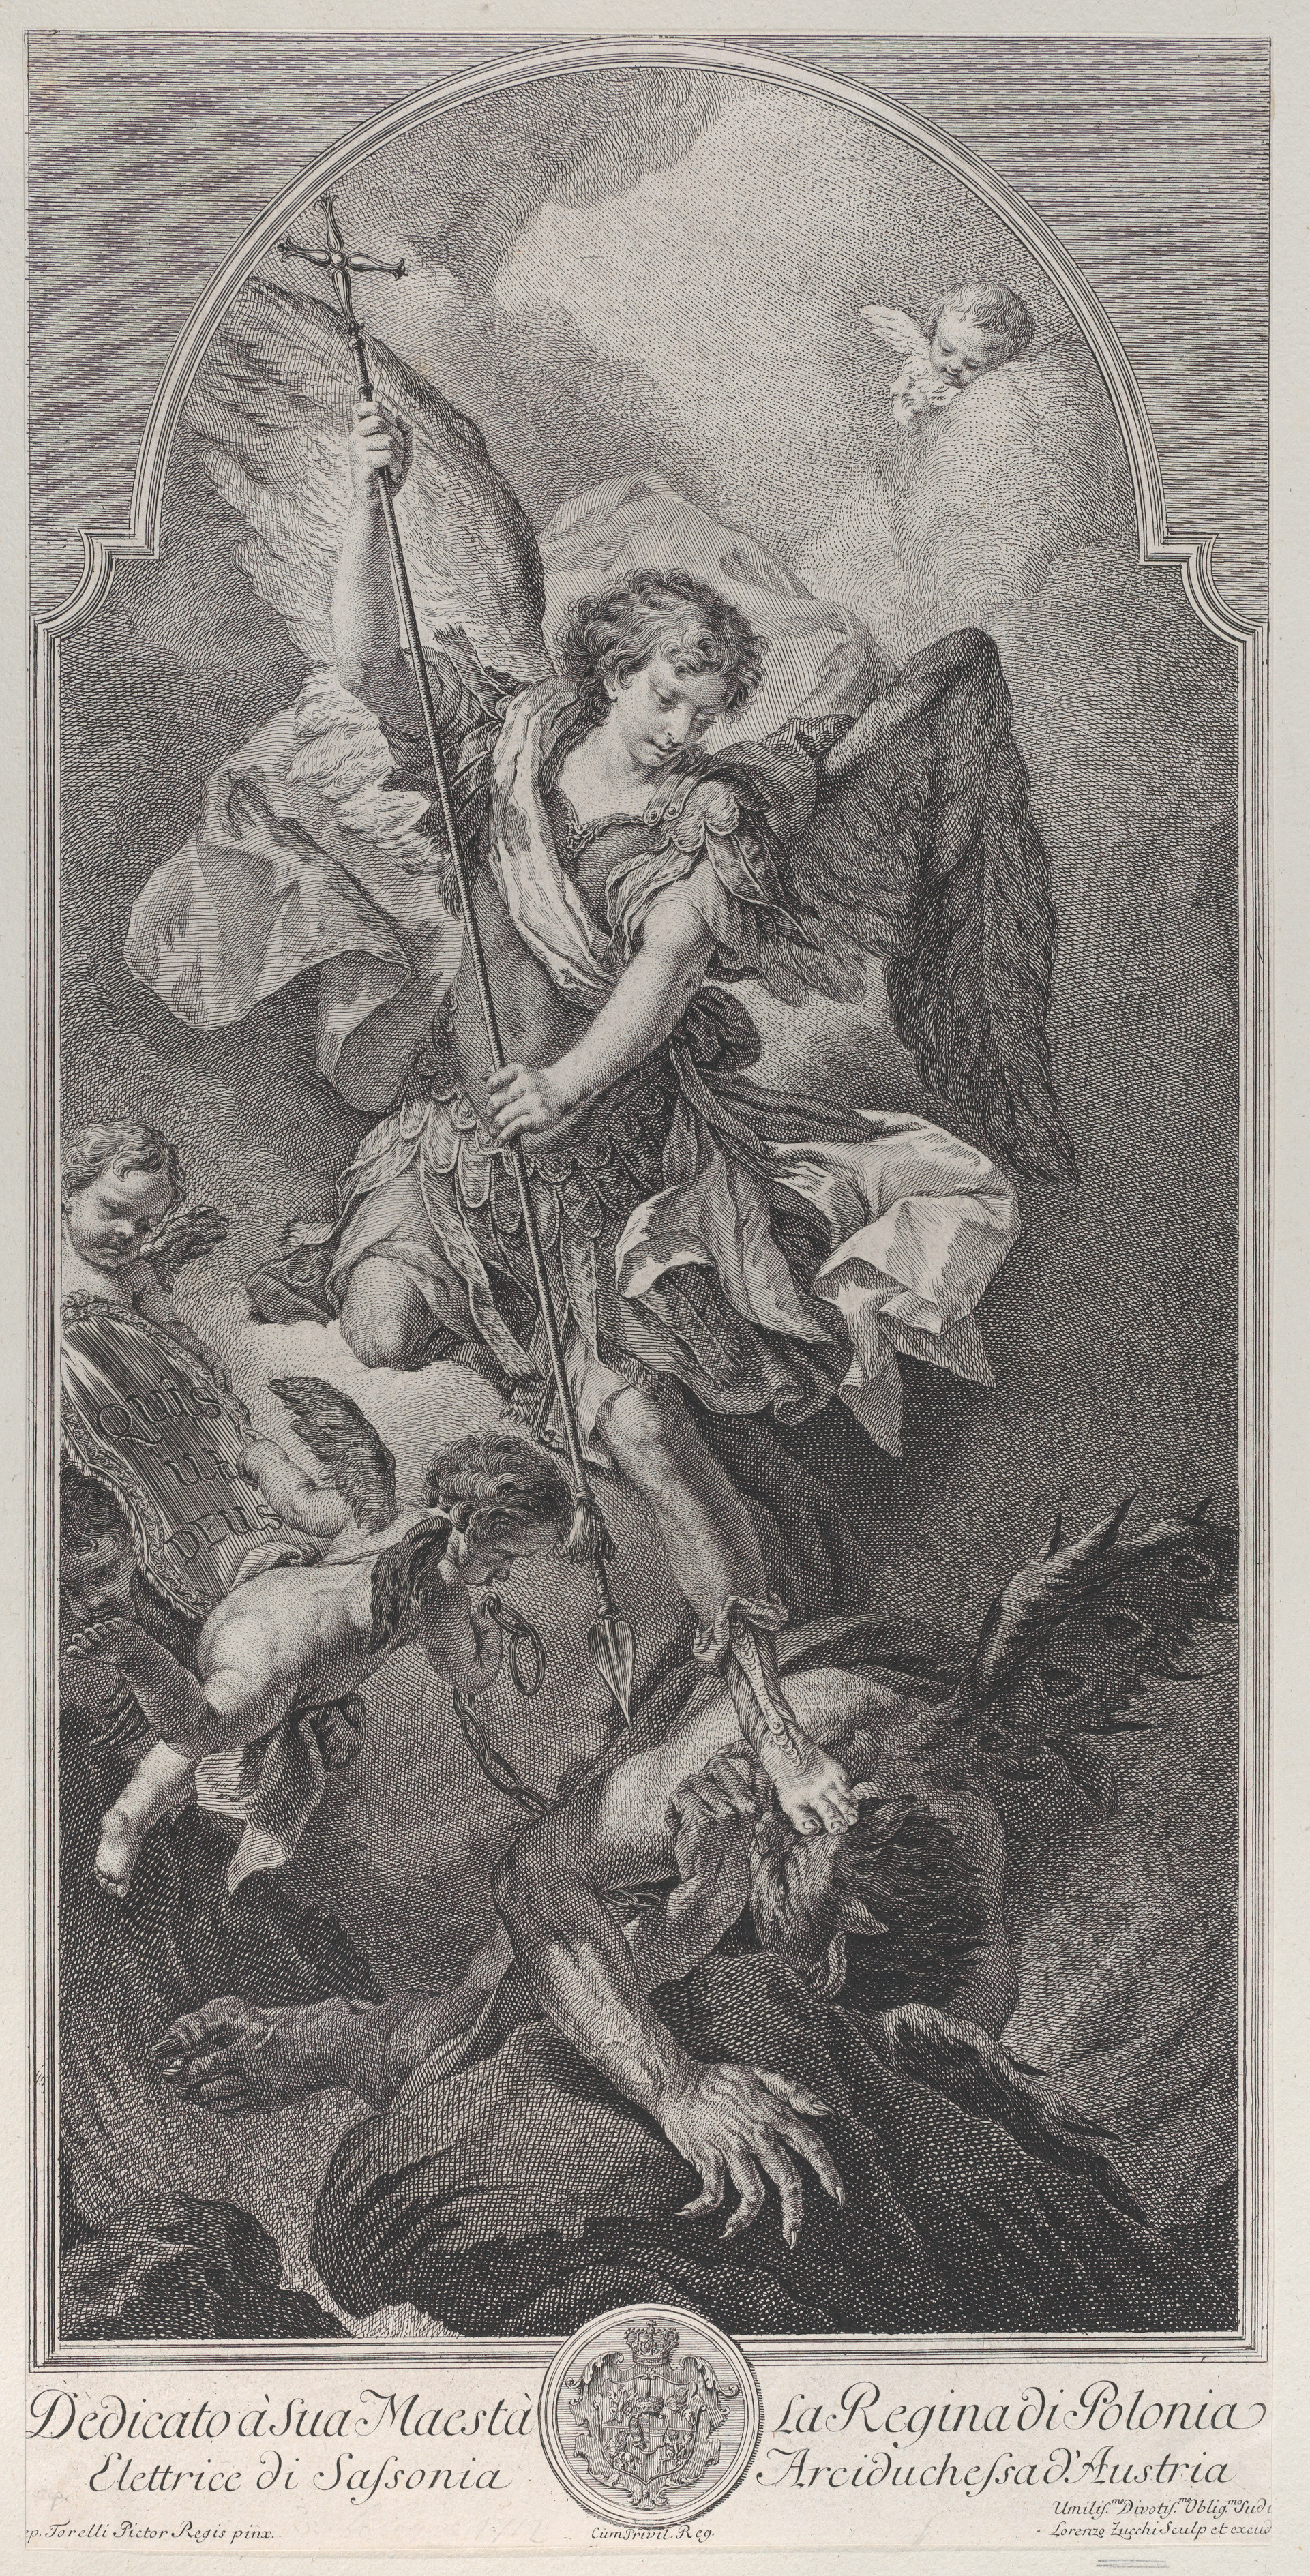
\includegraphics[height=0.75\textheight, keepaspectratio]{st_michael_defeating_satan.jpg}
	\caption{Saint Michael defeating Satan \cite{met_michael}}
	\label{fig:st_michael}
\end{figure}
\rubric{The Petition}

\begingroup
\centering
% LATIN
{\latinfont\Large
	Sáncte Míchael Archángele, defénde nos in proélio; \par
	contra nequítiam et insídias diáboli esto praesídium. \par
	Imperet illi Deus, súpplices deprecámur: \par
	tuque, Prínceps milítiae caeléstis, \par
	Sátanam aliósque spíritus malígnos, \par
	qui ad perditiónem animárum pervagántur in mundo, \par
	divína virtúte, in inférnum detrúde. \par
	Amen. \rubriccross \par
}

\vspace{1em}

% ENGLISH
{\itshape\small
	Saint Michael the Archangel, defend us in battle.
	Be our protection against the wickedness and snares of the devil;
	May God rebuke him, we humbly pray;
	and do thou, O Prince of the Heavenly Host, by the power of God,
	cast into hell Satan and all evil spirits
	who wander through the world for the ruin of souls.
	Amen. \par}
\endgroup

% ==========================================
% 4. THE LONG FORM EXORCISM
% ==========================================
\subsection{The Exorcismus in Satanam}
The long form exorcism prayer composed by Pope Leo XIII in 1890. This is reserved for use by bishops and authorized priests.

% --- MOVEMENT 1: THE INVOCATION ---
\rubric{The Invocation}
\textit{\small To be recited standing, with the Sign of the Cross made where indicated.}

\begingroup
\centering
% LATIN
{\latinfont\large
	In nómine Iesu Christi, Dei et Dómini nostri, \par
	intercessióne Immaculátæ Vírginis Dei Genetrícis Maríæ \rubriccross, \par
	Beáti Michaélis Archángeli \rubriccross, \par
	Beáti Ioánnis Baptístæ \rubriccross, \par
	Sanctórum Apostolórum Petri et Páuli \rubriccross, \par
	et ómnium Sanctórum, \par
	fidúcia ministérii nostri sacri, \par
	adversus versútias et insídias diáboli cum fidúcia aggredímur. \par}

\vspace{0.5em}

% ENGLISH
{\itshape\small
	In the Name of Jesus Christ, our God and Lord,
	strengthened by the intercession of the Immaculate Virgin Mary, Mother of God,
	of Blessed Michael the Archangel, of the Blessed Apostles Peter and Paul and all the Saints,
	and powerful in the holy authority of our ministry,
	we confidently undertake to repulse the attacks and deceits of the devil.\par}
\endgroup

\vspace{1.5em}

% --- MOVEMENT 2: THE PSALM (Psalm 67) ---
\rubric{Psalm 67 (Exsurgat Deus)}

\begingroup
\centering
{\latinfont\large
	Exsúrgat Deus, et dissipéntur inimíci eius: \par
	et fúgiant qui odérunt eum a fácie eius. \par
	Sicut déficit fumus defíciant; \par
	sicut fluit cera a fácie ígnis, \par
	sic péreant peccatóres a fácie Dei. \par}

\vspace{0.5em}

{\itshape\small
	God arises; His enemies are scattered and those who hate Him flee before Him.
	As smoke is driven away, so are they driven;
	as wax melts before the fire, so the wicked perish at the presence of God.\par}
\endgroup

\vspace{1.5em}

% --- MOVEMENT 3: THE COMMANDS ---
\rubric{The Commands}
\textit{\small The Exorcist commands the presence directly.}

\begingroup
\latinfont\large
\setlength{\parindent}{0pt}
\setlength{\parskip}{0.3em}

% Left-aligned (ragged right) for the 'Imperat' commands
Imperat tibi Deus Pater. \rubriccross \par
Imperat tibi Deus Fílius. \rubriccross \par
Imperat tibi Deus Spíritus Sanctus. \rubriccross \par
Imperat tibi Maiéstas Christi, Verbum Dei incarnátum. \rubriccross \par
Imperat tibi Virgo gloriósa, Dei Genetrix María. \rubriccross \par
Imperat tibi fides Sanctórum Apostolórum Petri et Páuli et aliórum Apostolórum. \rubriccross \par
Imperat tibi sanguis Mártyrum, imperat tibi pia intercessió Sanctorum et Sanctárum. \rubriccross \par
\endgroup

\vspace{0.5em}

\begin{quote}
	\itshape\small
	God the Father commands you.
	God the Son commands you. God the Holy Ghost commands you.
	Christ, God's Word made flesh, commands you.
	The glorious Mother of God, the Virgin Mary, commands you.
	The faith of the holy Apostles Peter and Paul, and of the other Apostles commands you.
	The blood of the Martyrs and the pious intercession of all the Saints command you.
\end{quote}

\vspace{1.5em}

% --- MOVEMENT 4: THE FINAL PRAYER (Missing Section) ---
\rubric{The Petition (Deus Caeli)}

\begingroup
\centering
{\latinfont\large
	Deus caeli, Deus terrae, \par
	Deus Angelórum, Deus Archangelórum, \par
	Deus qui potestátem habes donáre vitam post mortem, \par
	réquiem post labórem: \par
	quia non est Deus praeter te, \par
	nec esse potest nisi tu, Creátor ómnium visibílium et invisibílium, \par
	cuius regni non erit finis: \par
	humíliter maiestáti glóriae tuae supplicámus, \par
	ut omni potestáte infernálium spirítuum, \par
	ab ómnibus insídiis, decéptio, nequítia et furóre eórum, \par
	nos poténter liberáre, et incólumes custodíre dignéris. \par
	Per Christum Dóminum nostrum. Amen. \rubriccross \par}

\vspace{0.5em}

{\itshape\small
	God of heaven, God of earth, God of Angels, God of Archangels,
	God who has the power to give life after death and rest after work:
	because there is no other God beside Thee, nor can there be,
	Creator of all things visible and invisible, of whose kingdom there shall be no end:
	we humbly pray Thy glorious Majesty to powerfully deliver us
	from all the power, snares, deceits, wickedness, and fury of the infernal spirits,
	and to keep us safe and sound.
	Through Christ our Lord. Amen.\par}
\endgroup

\vspace{2em}
\hrule width 1.0\textwidth \relax
\vspace{2em}

    \appendix
    \setcounter{table}{0}
    \setcounter{figure}{0}
    \setcounter{page}{1}
    \renewcommand{\thetable}{A.\arabic{table}} 
    \renewcommand{\thefigure}{A.\arabic{figure}}
    \renewcommand{\thepage}{A.\arabic{page}}

    	\section{PRONUNCIATION GUIDE}
	\subsection{Sumero-Akkadian Phonetics}
	The following diacritical marks are used in the transcription of the Fifty Names to ensure correct pronunciation of the divine vibrations.
	
	\begin{xltabular}{\textwidth}{|c|l|X|}
		\hline
		\textbf{Symbol} & \textbf{Sound} & \textbf{Example} \\ \hline
		\endhead
		\v{s} & \textbf{sh} as in \textit{ship} & \textsc{\v{S}azu} (pronounced \textit{Shah-zoo}) \\ \hline
		\d{h} & \textbf{ch} as in Scottish \textit{loch} & \textsc{Asallu\d{h}i} (pronounced \textit{Ah-sall-oo-khee}) \\ \hline
		\d{t} & Emphatic \textbf{t}, hard stop & \textit{\d{T}uppu} (Tablet) \\ \hline		\d{s} & Emphatic \textbf{s} (ts sound) & \textit{Mu\d{s}a\d{s}ir} \\ \hline
		\={a}, \={e}, \={u} & Long vowels, held for double duration & \textit{E\={n}\={u}ma Eli\v{s}} \\ \hline
		\caption{Sumero-Akkadian Phonetics}
		\label{tab:pronunciation}
	\end{xltabular}


    	\section{MATERIALS AND TIMING}
	\subsection{Metals and Their Uses}
		\begin{xltabular}{\textwidth}{|X|X|X|X|}
			\hline
			\textbf{Metal} & \textbf{Planet} & \textbf{Property} & \textbf{Use in Defense} \\ \hline
			\endhead
			Lead   & Saturn & Restriction, binding  & Trapping seals, vessel lids \\ \hline
			Iron   & Mars   & Aggression, repulsion  & Threshold nails, blades     \\ \hline
			Silver & Moon   & Reflection, purity     & Pentagram pendants          \\ \hline
			Copper & Venus  & Conductivity, harmony  & Circle inscriptions         \\ \hline
			Brass  & ---    & Containment            & Binding vessels             \\ 		\hline
			\caption{Metals and Their Uses}
			\label{tab:metals} \\
		\end{xltabular}
	\subsection{Incenses}
		\begin{xltabular}{\textwidth}{|l|X|}
			\hline
			\textbf{Purpose} & \textbf{Incense} \\ \hline
			\endhead
			Purification & Frankincense \\ \hline
			Authority/Command & Frankincense + mastic \\ \hline
			Repulsion & Asafoetida, sulfur, black pepper \\ \hline
			Binding & Myrrh + sulfur \\ \hline
			Sealing & Benzoin \\ \hline
			\caption{Incenses}
	\label{tab:incenses}\\
		\end{xltabular}
	\subsection{Timing}
	Optimal conditions for defensive work:
	\begin{itemize}
		\item Moon phase: Waning (for banishing/repulsion) or Dark (for binding/trapping)
		\item Day: Saturday (Saturn---binding, endings) or Tuesday (Mars---aggressive action)
		\item Hour: Saturn hour for binding; Mars hour for repulsion; Sun hour for authority
		\item Moon sign: Earth signs (Taurus, Virgo, Capricorn) for permanence
	\end{itemize}


    	\section{QUICK REFERENCE PROCEDURE}
	\subsection{Complete Procedure Checklist}
	PREPARATION
	
	\begin{enumerate}
		\item Timing: Waning/dark moon, Saturday/Tuesday, Saturn/Mars hour
		\item Personal cleansing and protection (salt bath, white garment, Pentagram)
		\item Circle of Solomon established
		\item Materials gathered: hazel wand, iron blade/nails, salt, holy water, incenses, candles
	\end{enumerate}
	CONSTRAINT
	
	\begin{enumerate}
		\item Triangle of Art placed over affected area
		\item Iron nails at corners
		\item Black candles lit
		\item Constraint formula spoken
	\end{enumerate}
	EXPULSION
	
	\begin{enumerate}
		\item First Conjuration (command)
		\item Second Conjuration (threat) --- if needed
		\item Third Conjuration (curse) --- if needed
		\item Physical severance with iron
		\item Recitation of Marduk names (optional layer)
		\item Vade Retro Satana / St.  Michael prayer (optional layer)
	\end{enumerate}
	CLEANSING
	
	\begin{itemize}
		\item Purification incense (frankincense, benzoin, camphor)
		\item Salt water throughout
		\item All corners and thresholds addressed
	\end{itemize}
	RECONSECRATION
	
	\begin{itemize}
		\item White candle circuit (clockwise)
		\item Hexagram placed at center
		\item Quarters sealed with pentagrams
		\item Protective installations in place
	\end{itemize}
	\subsection[Emergency Short{}-Form Procedure]{Emergency Short-Form Procedure}
	When full ritual isn't possible:
	
	\begin{itemize}
		\item Hold iron object (nail, blade, key)
		\item Speak firmly: \enquote{By TETRAGRAMMATON, thou art commanded.  By ADONAI, thou art expelled.  By AGLA, thou art barred from return.  DEPART NOW.}
		\item Cast salt toward disturbance
		\item Trace pentagram in air, speak \enquote{AGLA} as you complete it
		\item Repeat as needed, increasing intensity
		\item Add: \enquote{Vade retro satana!} and/or St.  Michael prayer
	\end{itemize}


    	\addtocontents{lof}{\protect\addvspace{10pt}}
	\addtocontents{lof}{\protect\contentsline{figure}{\textbf{Full Size Figures}}{}{}}
	
	
	\section{Full Size Images}
	\begin{figure}[H]
		\centering
		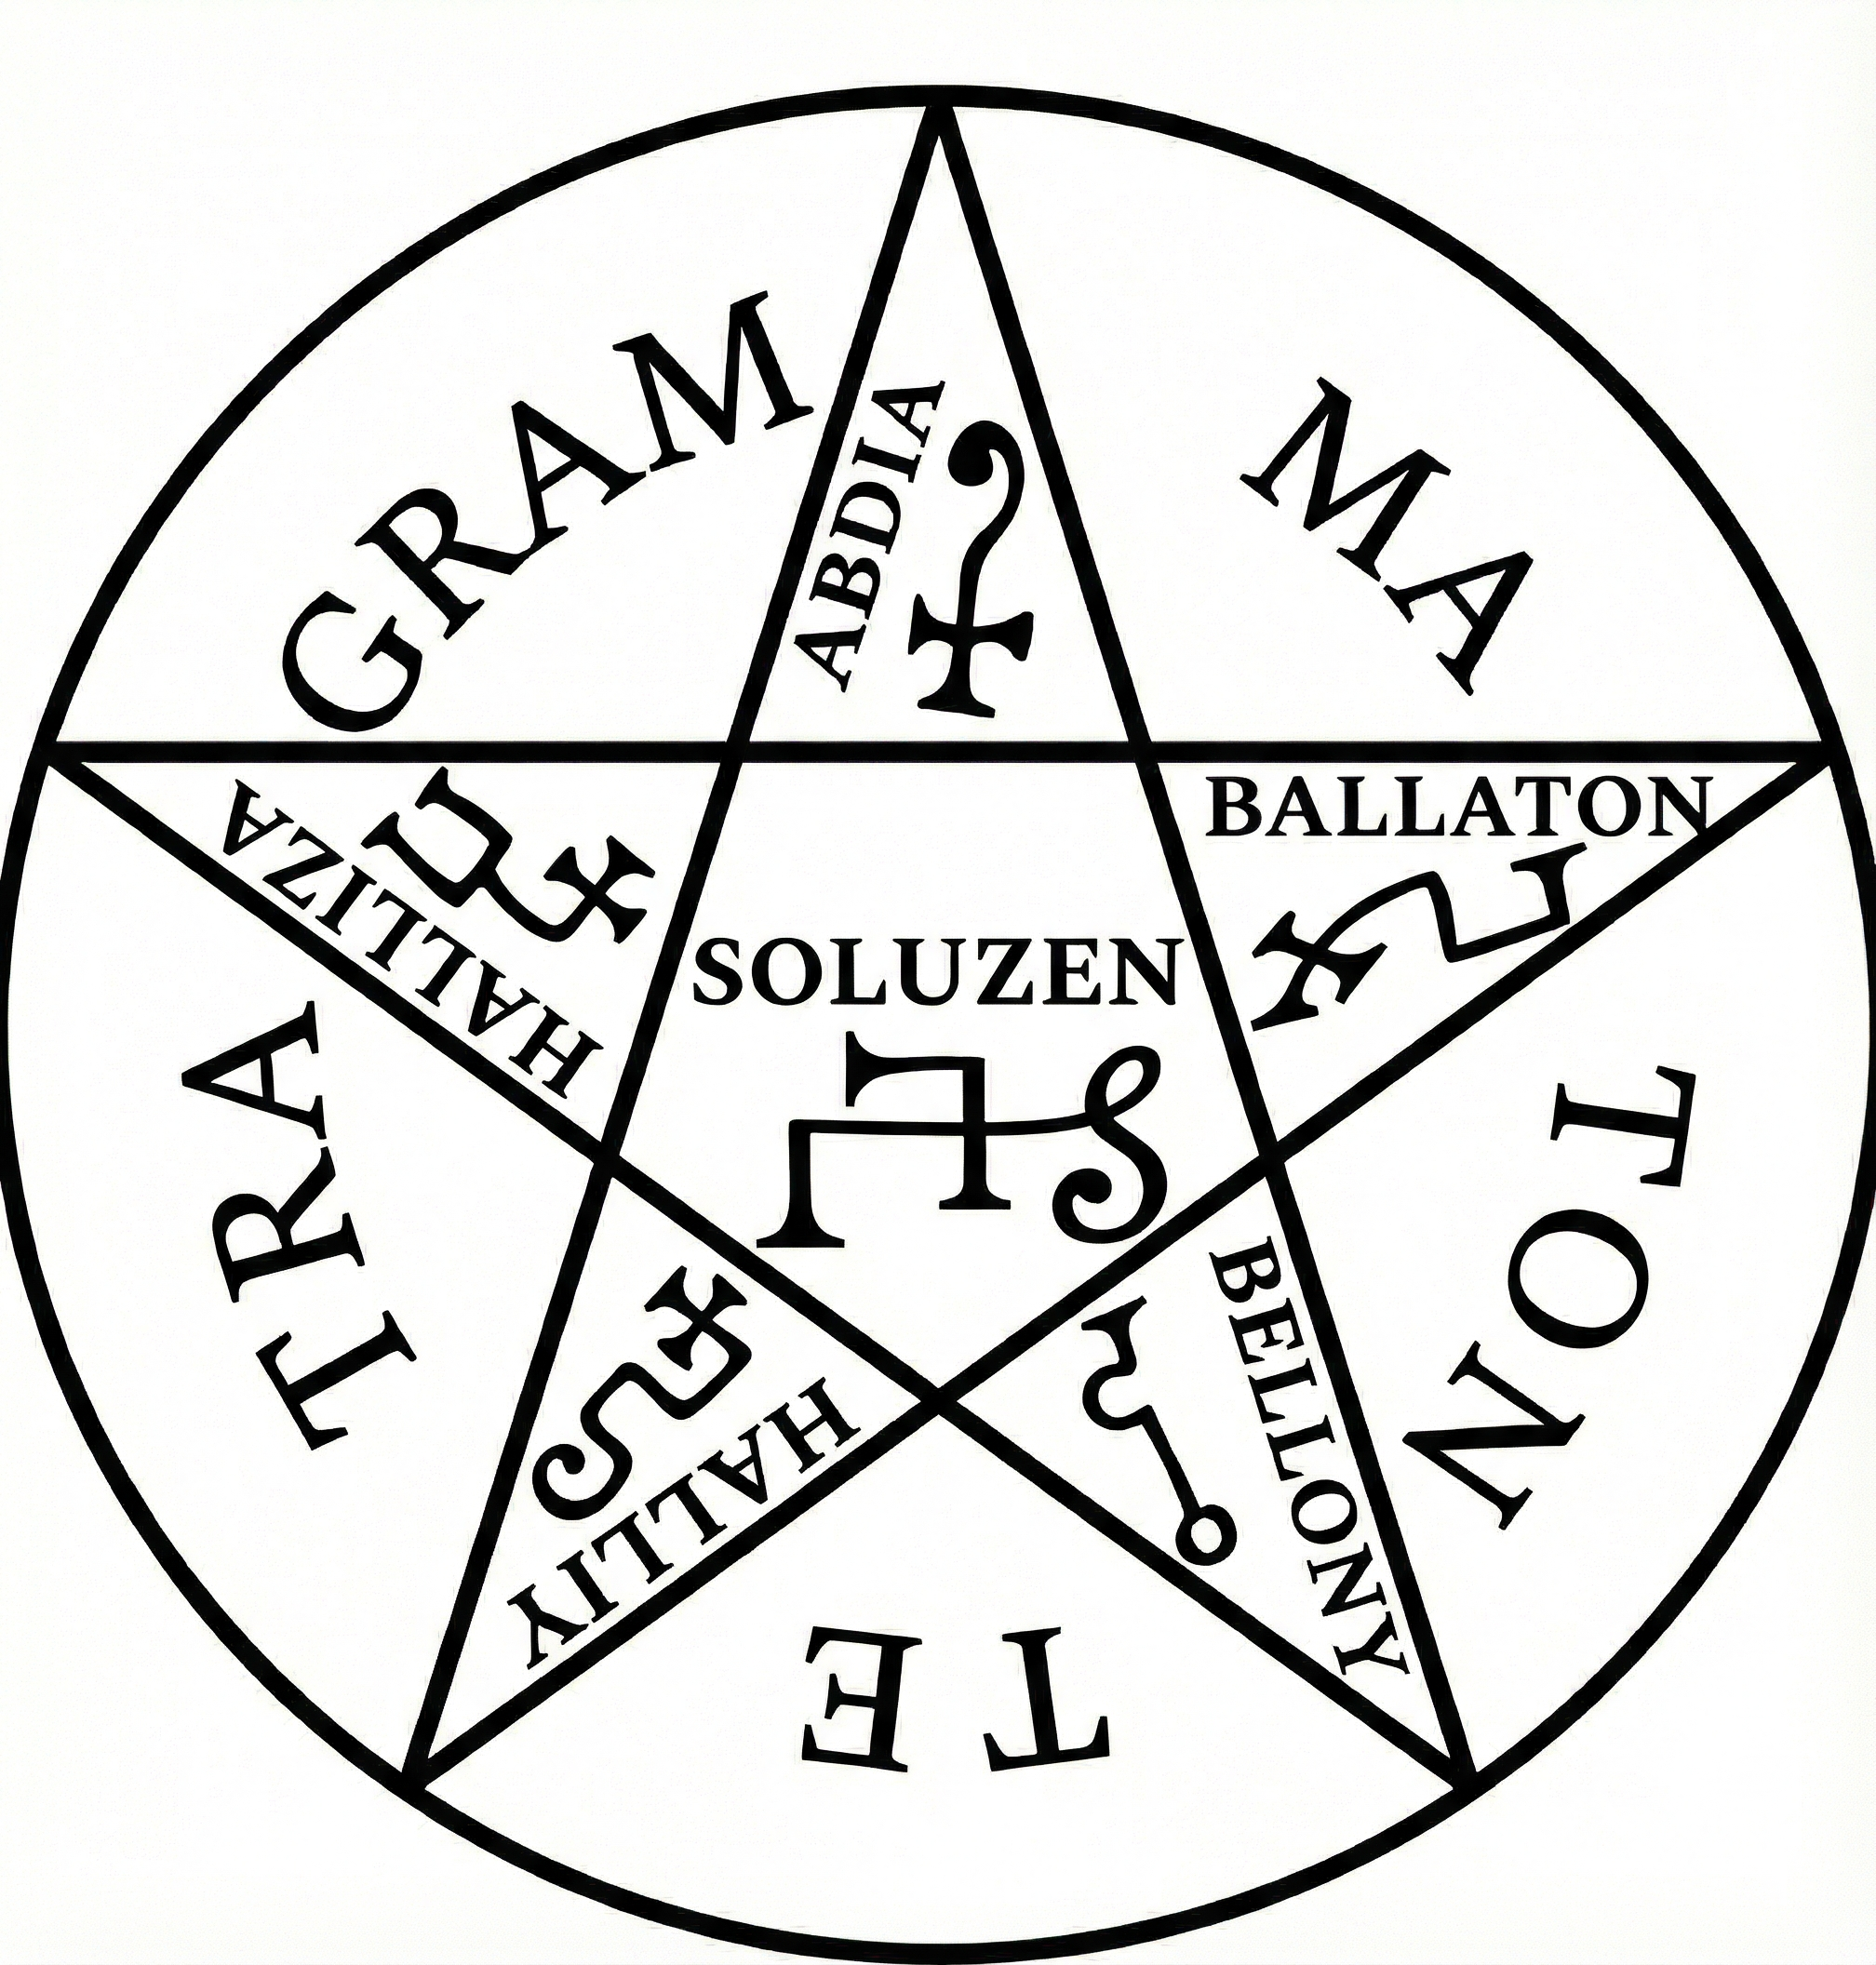
\includegraphics[width=0.8\textwidth,height=0.8\textheight,keepaspectratio]{solomon_pentagram.png}
		\caption{The Pentagram of Solomon}
		\label{fig:solomonpentagramfull}
	\end{figure}

	\clearpage
	\begin{figure}[p]
		\centering
		\includegraphics[width=0.8\textwidth,keepaspectratio]{solomon_hexagram.png}
		\caption{The Hexagram of Solomon}
		\label{fig:solomonhexagramfull}
	\end{figure}

	\clearpage
	\begin{figure}[p]
		\centering
		\includegraphics[width=0.8\textwidth,keepaspectratio]{solomon_triangle.png}
		\caption{The Triangle of Art}
		\label{fig:solomontrianglefull}
	\end{figure}

	\clearpage
	\begin{figure}[p]
		\centering
		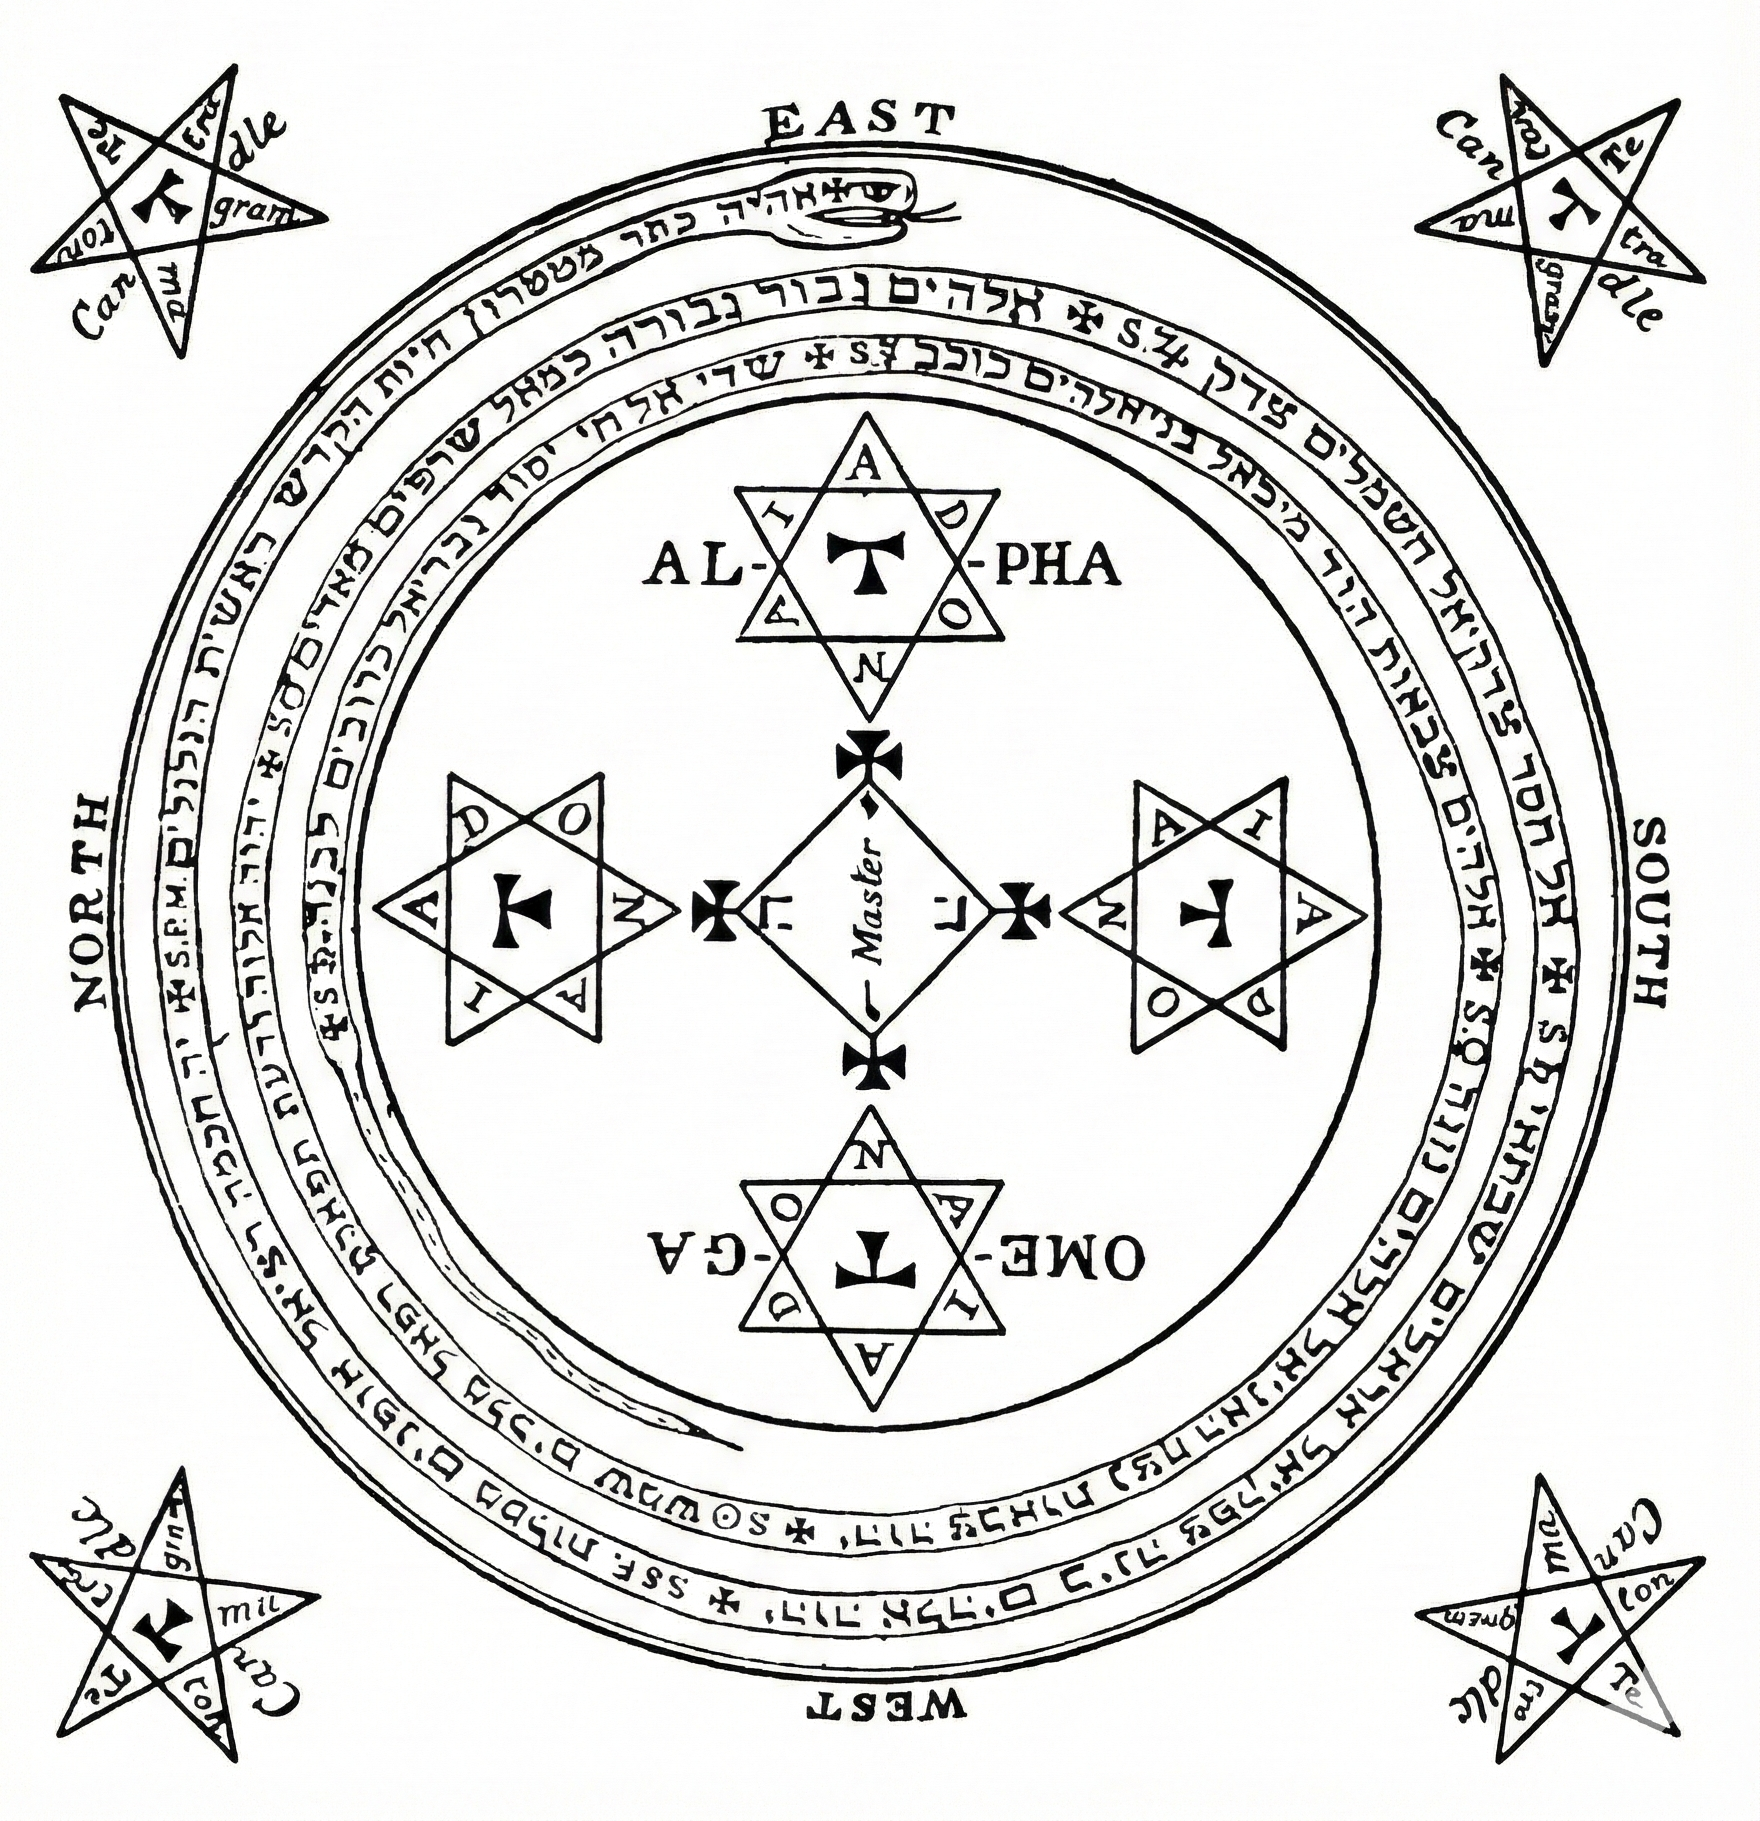
\includegraphics[width=0.8\textwidth,keepaspectratio]{solomon_circle.png}
		\caption{The Circle of Solomon}
		\label{fig:solomoncirclefull}
	\end{figure}

	\clearpage
	\begin{figure}[p]
		\centering
		\includegraphics[width=0.8\textwidth,keepaspectratio]{solomon_circle_and_triangle.png}
		\caption{Circle and Triangle}
		\label{fig:solomonfrontfull}
	\end{figure}

	\clearpage
	\begin{figure}[p]
		\centering
		\includegraphics[width=0.8\textwidth,keepaspectratio]{benedict_face.png}
		\caption{Detail of the Front Inscription (Crux S. Patris Benedicti) \cite{stutler_medal}}
		\label{fig:benedictfrontfull}
	\end{figure}

	\clearpage
	\begin{figure}[p]
		\centering
		\includegraphics[width=0.8\textwidth,keepaspectratio]{benedict_cross.png}
		\caption{Detail of the Reverse Inscription (Crux S. Patris Benedicti) \cite{stutler_medal}}
		\label{fig:benedictcrossfull}
	\end{figure}
	
	\clearpage
	\begin{figure}[p]
		\centering
		\includegraphics[width=0.8\textwidth,keepaspectratio]{st_anthony_brief_shield.png}
		\caption{Saint Anthony's Brief on a Shield}
		\label{fig:st_anthony_brief_full}
	\end{figure}

	\fullsizeimage{st_anthony_brief_cross.jpg}{Cruciform Brief of Saint Anthony}{c. 1880.  Private Collection}{anthony_brief_source}

	\clearpage
	\begin{figure}[p]
		\centering
		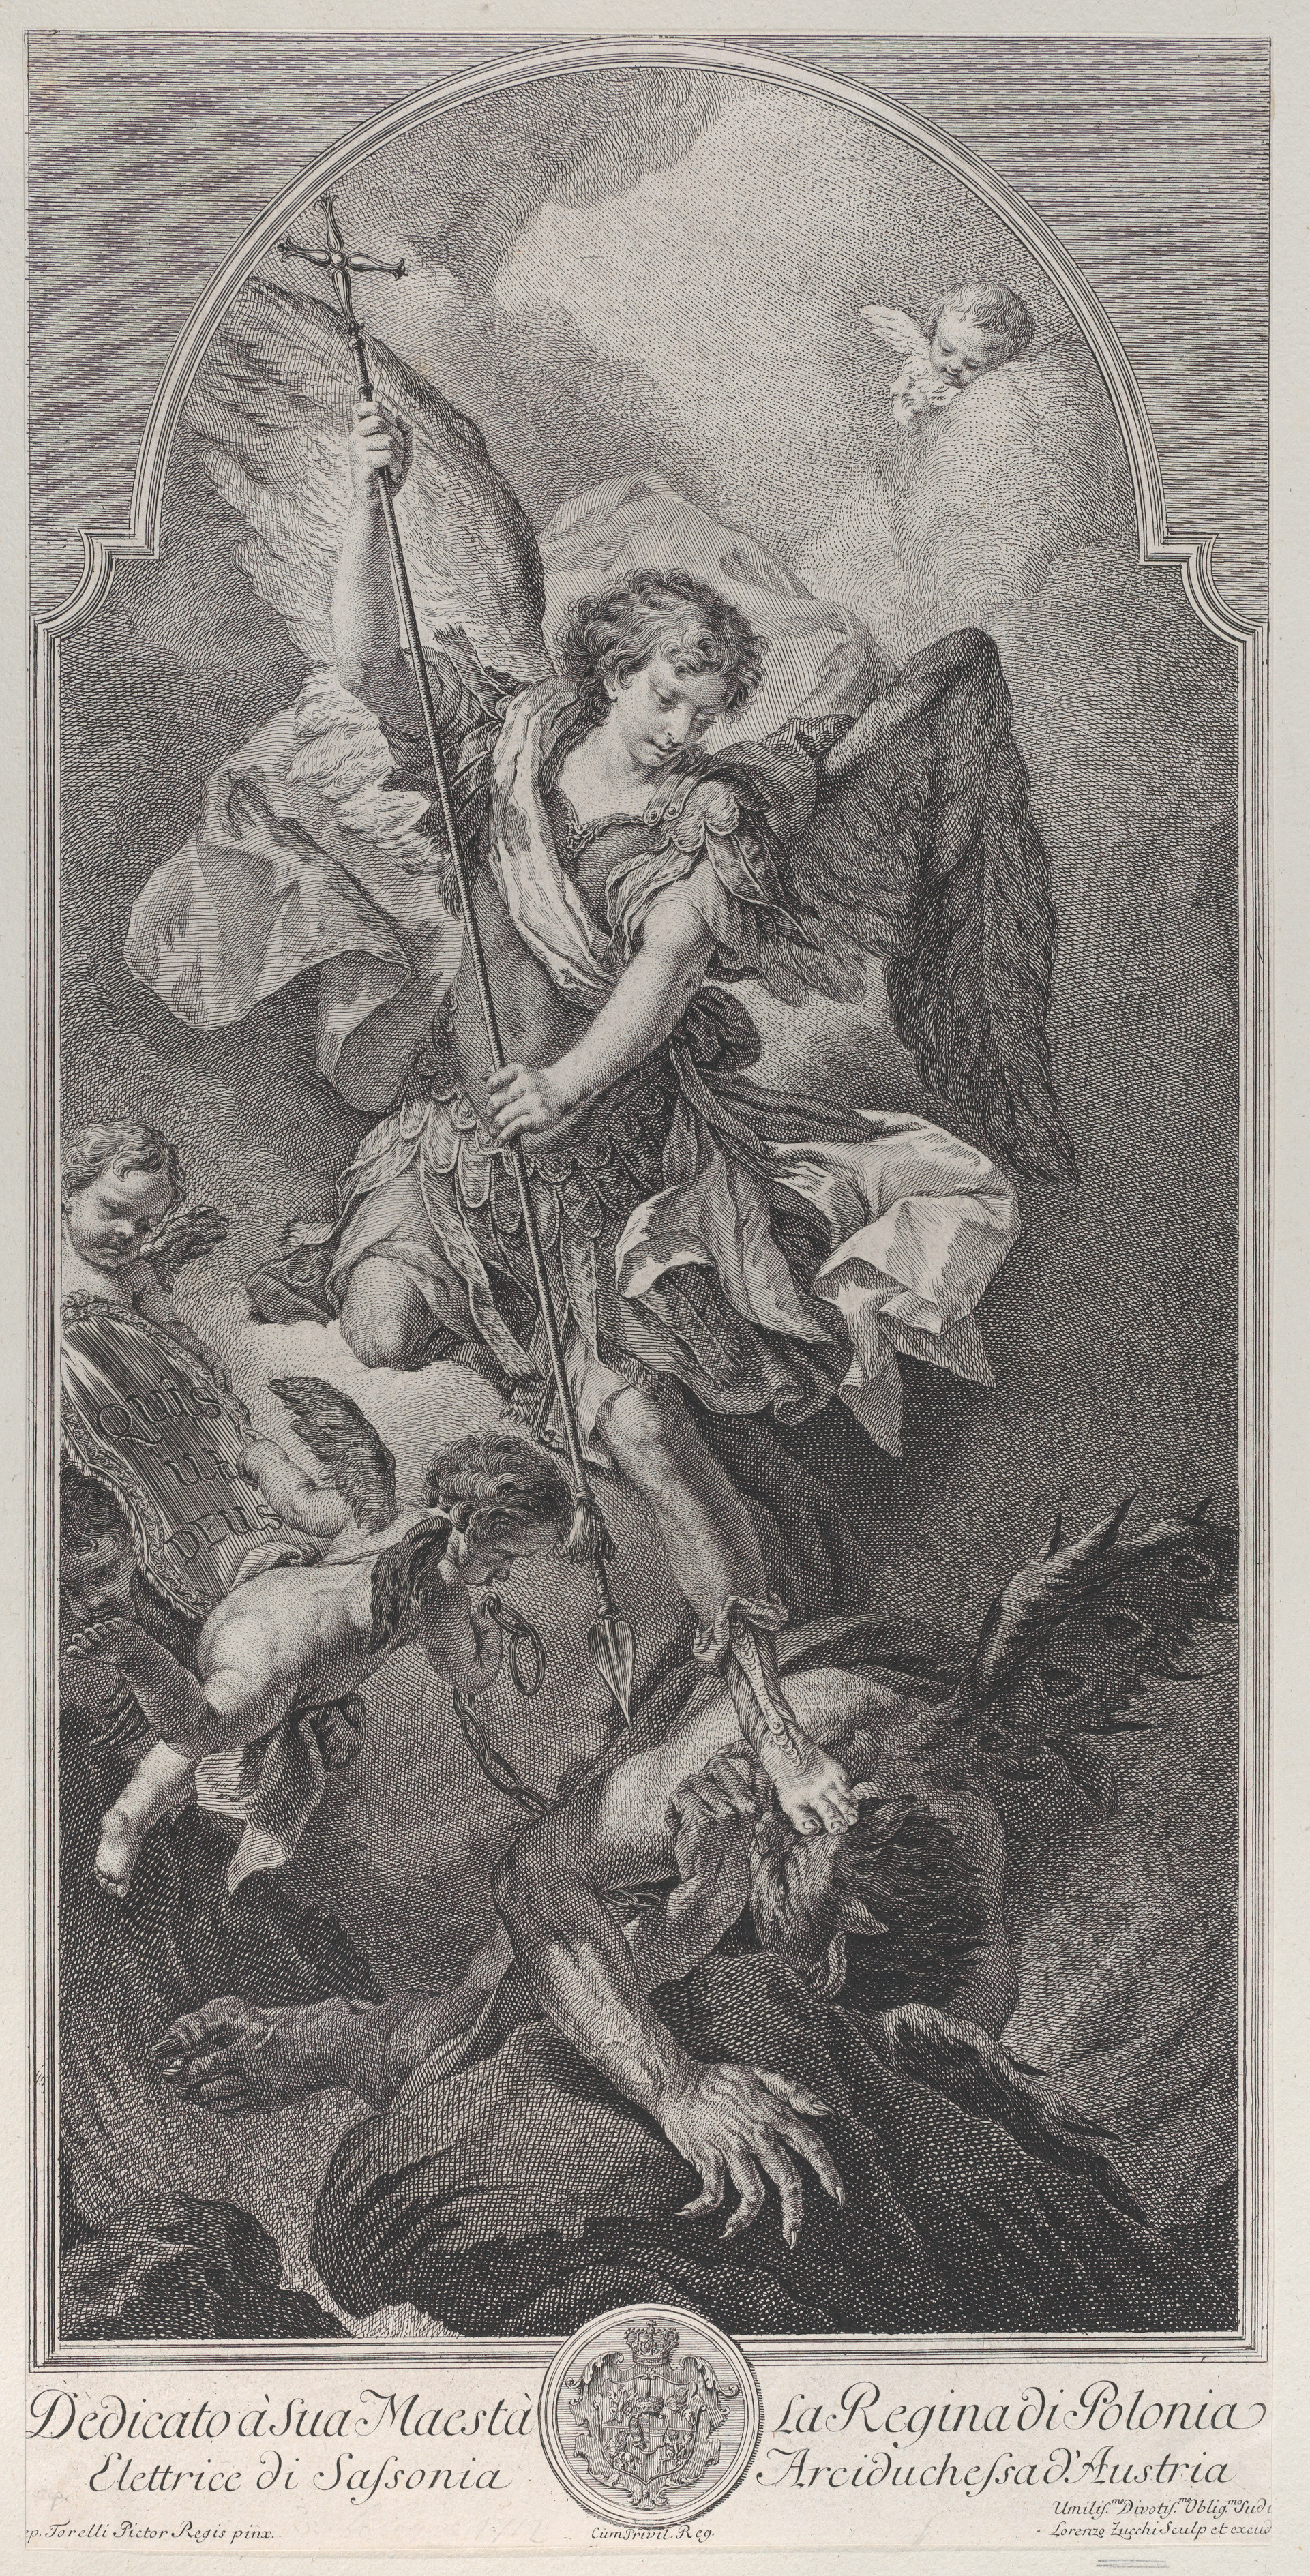
\includegraphics[width=0.9\textwidth,height=0.9\textheight, keepaspectratio]{st_michael_defeating_satan.jpg}

		\caption[St. Michael Detail]{The Archangel Michael defeats Satan.\\
		\textit{Lorenzo Zucchi (Italian, 1725--1779). Engraving after Stefano Torelli.}}

		% \nocite ensures it is still in the bibliography list, even though we didn't use brackets here
		\nocite{met_michael}
		\label{fig:st_michael_full}
	\end{figure}
	
	\fullsizeimage{tobias_woodcut.jpg}{Tobias Catching the Fish}{Ninth German Bible (Anton Koberger, 1483)}{koberger_bible}
	


	% Closing page
	\clearpage
\thispagestyle{empty} % No page number for the final seal

\vspace*{\fill}

\begin{center}
	{\Huge \textsc{Finis}} \\
	\vspace{2cm}
	
	\begin{minipage}{0.75\textwidth}
		\centering
		\itshape
		\large
		By the authority of the divine names, \\
		may this work serve those who seek protection.
	\end{minipage}
	
	\vspace{2cm}
	
	\textbullet \quad \textsc{Tetragrammaton} \quad \textbullet \\
	\vspace{0.5em}
	\textsc{Adonai} \quad \textbullet \quad \textsc{Agla} \\
	\vspace{0.5em}
	\textsc{Marduk} \quad \textbullet \quad \textsc{Michael}
	
\end{center}

\vspace*{\fill}
    % BACK MATTER
    % \nocite{*} 
    \printbibliography[keyword=babylonian,title={Sources for Babylonian Rituals}]
    \printbibliography[keyword=catholic,title={Sources for Catholic Liturgical Texts}]
    \printbibliography[keyword=occult,title={Sources for Occult Literature}]
    
    \printglossaries
    \printindex

\end{document}
